\section{Wyznaczenie symulacyjne odpowiedzi skokowych}
\label{projekt:zad2}

-------POLECENIE--------

Wyznaczyc symulacyjnie odpowiedzi skokowe torów wejscie-wyjscie i zakłócenie-wyjscie
procesu dla kilku zmian sygnału sterujacego. Narysowac te odpowiedzi, oddzielnie dla
obydwu torów. Narysowac charakterystyke statyczna procesu y(u, z). Czy własciwosci
statyczne i dynamiczne procesu sa (w przyblizeniu) liniowe? Jezeli tak, okreslic
wzmocnienie statyczne obu torów procesu.

-------POLECENIE--------


Odpowiedzi skokowe torów wejście-wyjście i zakłócenie-wyjście zostały wyznaczone
symulacyjnie dla pięciu zmian sygnału sterującego oraz pięciu zmian zakłócenia .

\subsection{Odpowiedź wyjścia na skok wejścia}
\label{projekt:zad2:StepYU}

Do uzyskania odpowiedzi skokowych dla tego toru ustawiono zakłócenie na stałą
wartość Z=0 oraz przeprowadzone zostały skoki sterowania z Upp =0 na …

\begin{figure}[H] 
    \centering
    % This file was created by matlab2tikz.
%
\definecolor{mycolor1}{rgb}{0.00000,0.44700,0.74100}%
\definecolor{mycolor2}{rgb}{0.85000,0.32500,0.09800}%
\definecolor{mycolor3}{rgb}{0.92900,0.69400,0.12500}%
\definecolor{mycolor4}{rgb}{0.49400,0.18400,0.55600}%
\definecolor{mycolor5}{rgb}{0.46600,0.67400,0.18800}%
%
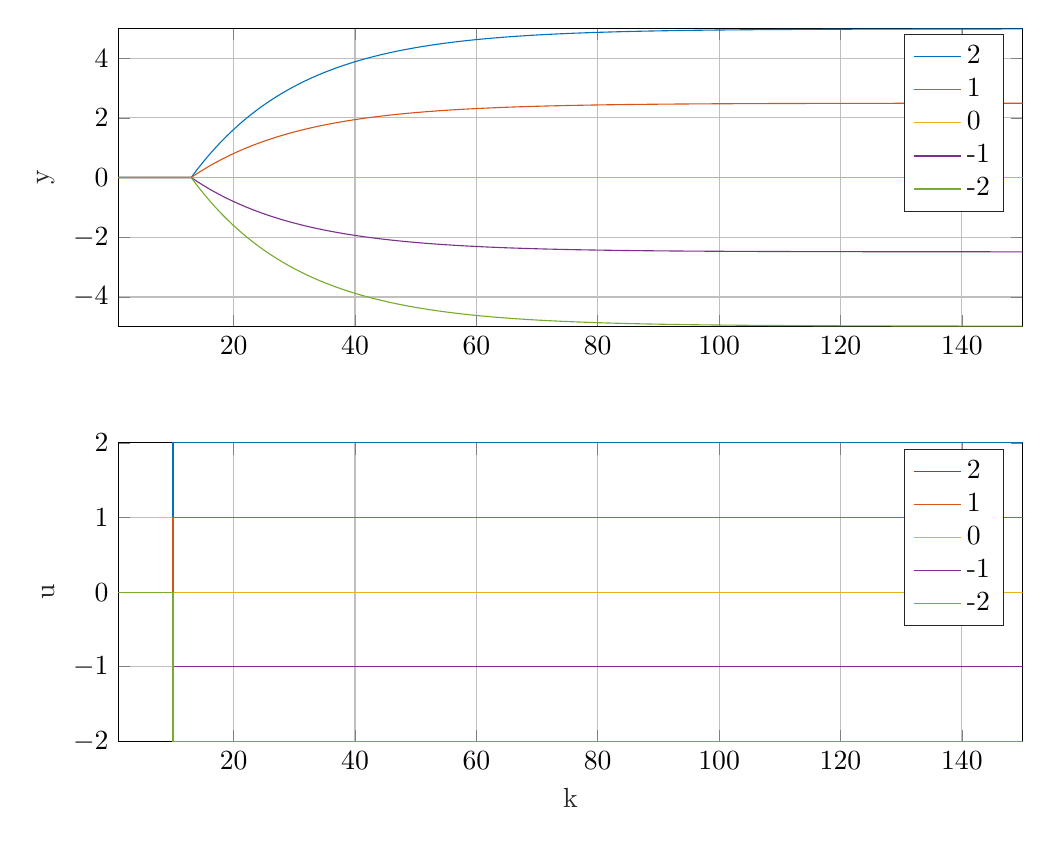
\begin{tikzpicture}

\begin{axis}[%
width=4.521in,
height=1.493in,
at={(0.758in,2.554in)},
scale only axis,
xmin=1,
xmax=150,
ymin=-5,
ymax=5,
ylabel style={font=\color{white!15!black}},
ylabel={y},
axis background/.style={fill=white},
xmajorgrids,
ymajorgrids,
legend style={legend cell align=left, align=left, draw=white!15!black}
]
\addplot [color=mycolor1]
  table[row sep=crcr]{%
1	0\\
2	0\\
3	0\\
4	0\\
5	0\\
6	0\\
7	0\\
8	0\\
9	0\\
10	0\\
11	0\\
12	0\\
13	0\\
14	0.2702\\
15	0.52579\\
16	0.76754\\
17	0.99621\\
18	1.2125\\
19	1.4171\\
20	1.6106\\
21	1.7936\\
22	1.9666\\
23	2.1303\\
24	2.2851\\
25	2.4316\\
26	2.57\\
27	2.701\\
28	2.8248\\
29	2.942\\
30	3.0527\\
31	3.1575\\
32	3.2565\\
33	3.3502\\
34	3.4388\\
35	3.5225\\
36	3.6018\\
37	3.6767\\
38	3.7475\\
39	3.8145\\
40	3.8778\\
41	3.9377\\
42	3.9944\\
43	4.0479\\
44	4.0986\\
45	4.1465\\
46	4.1918\\
47	4.2346\\
48	4.2751\\
49	4.3134\\
50	4.3496\\
51	4.3838\\
52	4.4162\\
53	4.4468\\
54	4.4758\\
55	4.5031\\
56	4.529\\
57	4.5535\\
58	4.5766\\
59	4.5985\\
60	4.6192\\
61	4.6388\\
62	4.6573\\
63	4.6748\\
64	4.6913\\
65	4.707\\
66	4.7218\\
67	4.7357\\
68	4.749\\
69	4.7615\\
70	4.7733\\
71	4.7845\\
72	4.795\\
73	4.805\\
74	4.8145\\
75	4.8234\\
76	4.8319\\
77	4.8399\\
78	4.8474\\
79	4.8546\\
80	4.8613\\
81	4.8677\\
82	4.8738\\
83	4.8795\\
84	4.8849\\
85	4.89\\
86	4.8948\\
87	4.8994\\
88	4.9037\\
89	4.9078\\
90	4.9116\\
91	4.9153\\
92	4.9187\\
93	4.922\\
94	4.9251\\
95	4.928\\
96	4.9307\\
97	4.9334\\
98	4.9358\\
99	4.9382\\
100	4.9404\\
101	4.9424\\
102	4.9444\\
103	4.9463\\
104	4.948\\
105	4.9497\\
106	4.9513\\
107	4.9528\\
108	4.9542\\
109	4.9555\\
110	4.9568\\
111	4.958\\
112	4.9591\\
113	4.9602\\
114	4.9612\\
115	4.9621\\
116	4.963\\
117	4.9639\\
118	4.9647\\
119	4.9654\\
120	4.9662\\
121	4.9668\\
122	4.9675\\
123	4.9681\\
124	4.9687\\
125	4.9692\\
126	4.9697\\
127	4.9702\\
128	4.9707\\
129	4.9711\\
130	4.9715\\
131	4.9719\\
132	4.9723\\
133	4.9726\\
134	4.9729\\
135	4.9733\\
136	4.9736\\
137	4.9738\\
138	4.9741\\
139	4.9743\\
140	4.9746\\
141	4.9748\\
142	4.975\\
143	4.9752\\
144	4.9754\\
145	4.9756\\
146	4.9757\\
147	4.9759\\
148	4.976\\
149	4.9762\\
150	4.9763\\
151	4.9764\\
152	4.9766\\
153	4.9767\\
154	4.9768\\
155	4.9769\\
156	4.977\\
157	4.9771\\
158	4.9772\\
159	4.9772\\
160	4.9773\\
161	4.9774\\
162	4.9775\\
163	4.9775\\
164	4.9776\\
165	4.9776\\
166	4.9777\\
167	4.9778\\
168	4.9778\\
169	4.9778\\
170	4.9779\\
171	4.9779\\
172	4.978\\
173	4.978\\
174	4.978\\
175	4.9781\\
176	4.9781\\
177	4.9781\\
178	4.9782\\
179	4.9782\\
180	4.9782\\
181	4.9782\\
182	4.9783\\
183	4.9783\\
184	4.9783\\
185	4.9783\\
186	4.9783\\
187	4.9784\\
188	4.9784\\
189	4.9784\\
190	4.9784\\
191	4.9784\\
192	4.9784\\
193	4.9784\\
194	4.9785\\
195	4.9785\\
196	4.9785\\
197	4.9785\\
198	4.9785\\
199	4.9785\\
200	4.9785\\
201	4.9785\\
202	4.9785\\
203	4.9785\\
204	4.9785\\
205	4.9785\\
206	4.9786\\
207	4.9786\\
208	4.9786\\
209	4.9786\\
210	4.9786\\
211	4.9786\\
212	4.9786\\
213	4.9786\\
214	4.9786\\
215	4.9786\\
216	4.9786\\
217	4.9786\\
218	4.9786\\
219	4.9786\\
220	4.9786\\
221	4.9786\\
222	4.9786\\
223	4.9786\\
224	4.9786\\
225	4.9786\\
226	4.9786\\
227	4.9786\\
228	4.9786\\
229	4.9786\\
230	4.9786\\
231	4.9786\\
232	4.9786\\
233	4.9786\\
234	4.9786\\
235	4.9786\\
236	4.9786\\
237	4.9786\\
238	4.9786\\
239	4.9786\\
240	4.9786\\
241	4.9786\\
242	4.9786\\
243	4.9786\\
244	4.9786\\
245	4.9786\\
246	4.9786\\
247	4.9786\\
248	4.9786\\
249	4.9786\\
250	4.9786\\
251	4.9786\\
252	4.9786\\
253	4.9786\\
254	4.9786\\
255	4.9786\\
256	4.9786\\
257	4.9786\\
258	4.9786\\
259	4.9786\\
260	4.9786\\
261	4.9786\\
262	4.9786\\
263	4.9786\\
264	4.9786\\
265	4.9786\\
266	4.9787\\
267	4.9787\\
268	4.9787\\
269	4.9787\\
270	4.9787\\
271	4.9787\\
272	4.9787\\
273	4.9787\\
274	4.9787\\
275	4.9787\\
276	4.9787\\
277	4.9787\\
278	4.9787\\
279	4.9787\\
280	4.9787\\
281	4.9787\\
282	4.9787\\
283	4.9787\\
284	4.9787\\
285	4.9787\\
286	4.9787\\
287	4.9787\\
288	4.9787\\
289	4.9787\\
290	4.9787\\
291	4.9787\\
292	4.9787\\
293	4.9787\\
294	4.9787\\
295	4.9787\\
296	4.9787\\
297	4.9787\\
298	4.9787\\
299	4.9787\\
300	4.9787\\
};
\addlegendentry{2}

\addplot [color=mycolor2]
  table[row sep=crcr]{%
1	0\\
2	0\\
3	0\\
4	0\\
5	0\\
6	0\\
7	0\\
8	0\\
9	0\\
10	0\\
11	0\\
12	0\\
13	0\\
14	0.1351\\
15	0.26289\\
16	0.38377\\
17	0.49811\\
18	0.60625\\
19	0.70854\\
20	0.80528\\
21	0.89678\\
22	0.98332\\
23	1.0652\\
24	1.1426\\
25	1.2158\\
26	1.285\\
27	1.3505\\
28	1.4124\\
29	1.471\\
30	1.5264\\
31	1.5787\\
32	1.6283\\
33	1.6751\\
34	1.7194\\
35	1.7613\\
36	1.8009\\
37	1.8383\\
38	1.8737\\
39	1.9072\\
40	1.9389\\
41	1.9689\\
42	1.9972\\
43	2.024\\
44	2.0493\\
45	2.0732\\
46	2.0959\\
47	2.1173\\
48	2.1375\\
49	2.1567\\
50	2.1748\\
51	2.1919\\
52	2.2081\\
53	2.2234\\
54	2.2379\\
55	2.2516\\
56	2.2645\\
57	2.2768\\
58	2.2883\\
59	2.2993\\
60	2.3096\\
61	2.3194\\
62	2.3286\\
63	2.3374\\
64	2.3457\\
65	2.3535\\
66	2.3609\\
67	2.3679\\
68	2.3745\\
69	2.3807\\
70	2.3866\\
71	2.3922\\
72	2.3975\\
73	2.4025\\
74	2.4072\\
75	2.4117\\
76	2.4159\\
77	2.4199\\
78	2.4237\\
79	2.4273\\
80	2.4307\\
81	2.4339\\
82	2.4369\\
83	2.4397\\
84	2.4424\\
85	2.445\\
86	2.4474\\
87	2.4497\\
88	2.4518\\
89	2.4539\\
90	2.4558\\
91	2.4576\\
92	2.4594\\
93	2.461\\
94	2.4625\\
95	2.464\\
96	2.4654\\
97	2.4667\\
98	2.4679\\
99	2.4691\\
100	2.4702\\
101	2.4712\\
102	2.4722\\
103	2.4731\\
104	2.474\\
105	2.4749\\
106	2.4756\\
107	2.4764\\
108	2.4771\\
109	2.4778\\
110	2.4784\\
111	2.479\\
112	2.4795\\
113	2.4801\\
114	2.4806\\
115	2.4811\\
116	2.4815\\
117	2.4819\\
118	2.4823\\
119	2.4827\\
120	2.4831\\
121	2.4834\\
122	2.4837\\
123	2.484\\
124	2.4843\\
125	2.4846\\
126	2.4849\\
127	2.4851\\
128	2.4853\\
129	2.4856\\
130	2.4858\\
131	2.486\\
132	2.4861\\
133	2.4863\\
134	2.4865\\
135	2.4866\\
136	2.4868\\
137	2.4869\\
138	2.487\\
139	2.4872\\
140	2.4873\\
141	2.4874\\
142	2.4875\\
143	2.4876\\
144	2.4877\\
145	2.4878\\
146	2.4879\\
147	2.4879\\
148	2.488\\
149	2.4881\\
150	2.4882\\
151	2.4882\\
152	2.4883\\
153	2.4883\\
154	2.4884\\
155	2.4884\\
156	2.4885\\
157	2.4885\\
158	2.4886\\
159	2.4886\\
160	2.4887\\
161	2.4887\\
162	2.4887\\
163	2.4888\\
164	2.4888\\
165	2.4888\\
166	2.4889\\
167	2.4889\\
168	2.4889\\
169	2.4889\\
170	2.4889\\
171	2.489\\
172	2.489\\
173	2.489\\
174	2.489\\
175	2.489\\
176	2.4891\\
177	2.4891\\
178	2.4891\\
179	2.4891\\
180	2.4891\\
181	2.4891\\
182	2.4891\\
183	2.4891\\
184	2.4892\\
185	2.4892\\
186	2.4892\\
187	2.4892\\
188	2.4892\\
189	2.4892\\
190	2.4892\\
191	2.4892\\
192	2.4892\\
193	2.4892\\
194	2.4892\\
195	2.4892\\
196	2.4892\\
197	2.4892\\
198	2.4892\\
199	2.4893\\
200	2.4893\\
201	2.4893\\
202	2.4893\\
203	2.4893\\
204	2.4893\\
205	2.4893\\
206	2.4893\\
207	2.4893\\
208	2.4893\\
209	2.4893\\
210	2.4893\\
211	2.4893\\
212	2.4893\\
213	2.4893\\
214	2.4893\\
215	2.4893\\
216	2.4893\\
217	2.4893\\
218	2.4893\\
219	2.4893\\
220	2.4893\\
221	2.4893\\
222	2.4893\\
223	2.4893\\
224	2.4893\\
225	2.4893\\
226	2.4893\\
227	2.4893\\
228	2.4893\\
229	2.4893\\
230	2.4893\\
231	2.4893\\
232	2.4893\\
233	2.4893\\
234	2.4893\\
235	2.4893\\
236	2.4893\\
237	2.4893\\
238	2.4893\\
239	2.4893\\
240	2.4893\\
241	2.4893\\
242	2.4893\\
243	2.4893\\
244	2.4893\\
245	2.4893\\
246	2.4893\\
247	2.4893\\
248	2.4893\\
249	2.4893\\
250	2.4893\\
251	2.4893\\
252	2.4893\\
253	2.4893\\
254	2.4893\\
255	2.4893\\
256	2.4893\\
257	2.4893\\
258	2.4893\\
259	2.4893\\
260	2.4893\\
261	2.4893\\
262	2.4893\\
263	2.4893\\
264	2.4893\\
265	2.4893\\
266	2.4893\\
267	2.4893\\
268	2.4893\\
269	2.4893\\
270	2.4893\\
271	2.4893\\
272	2.4893\\
273	2.4893\\
274	2.4893\\
275	2.4893\\
276	2.4893\\
277	2.4893\\
278	2.4893\\
279	2.4893\\
280	2.4893\\
281	2.4893\\
282	2.4893\\
283	2.4893\\
284	2.4893\\
285	2.4893\\
286	2.4893\\
287	2.4893\\
288	2.4893\\
289	2.4893\\
290	2.4893\\
291	2.4893\\
292	2.4893\\
293	2.4893\\
294	2.4893\\
295	2.4893\\
296	2.4893\\
297	2.4893\\
298	2.4893\\
299	2.4893\\
300	2.4893\\
};
\addlegendentry{1}

\addplot [color=mycolor3]
  table[row sep=crcr]{%
1	0\\
2	0\\
3	0\\
4	0\\
5	0\\
6	0\\
7	0\\
8	0\\
9	0\\
10	0\\
11	0\\
12	0\\
13	0\\
14	0\\
15	0\\
16	0\\
17	0\\
18	0\\
19	0\\
20	0\\
21	0\\
22	0\\
23	0\\
24	0\\
25	0\\
26	0\\
27	0\\
28	0\\
29	0\\
30	0\\
31	0\\
32	0\\
33	0\\
34	0\\
35	0\\
36	0\\
37	0\\
38	0\\
39	0\\
40	0\\
41	0\\
42	0\\
43	0\\
44	0\\
45	0\\
46	0\\
47	0\\
48	0\\
49	0\\
50	0\\
51	0\\
52	0\\
53	0\\
54	0\\
55	0\\
56	0\\
57	0\\
58	0\\
59	0\\
60	0\\
61	0\\
62	0\\
63	0\\
64	0\\
65	0\\
66	0\\
67	0\\
68	0\\
69	0\\
70	0\\
71	0\\
72	0\\
73	0\\
74	0\\
75	0\\
76	0\\
77	0\\
78	0\\
79	0\\
80	0\\
81	0\\
82	0\\
83	0\\
84	0\\
85	0\\
86	0\\
87	0\\
88	0\\
89	0\\
90	0\\
91	0\\
92	0\\
93	0\\
94	0\\
95	0\\
96	0\\
97	0\\
98	0\\
99	0\\
100	0\\
101	0\\
102	0\\
103	0\\
104	0\\
105	0\\
106	0\\
107	0\\
108	0\\
109	0\\
110	0\\
111	0\\
112	0\\
113	0\\
114	0\\
115	0\\
116	0\\
117	0\\
118	0\\
119	0\\
120	0\\
121	0\\
122	0\\
123	0\\
124	0\\
125	0\\
126	0\\
127	0\\
128	0\\
129	0\\
130	0\\
131	0\\
132	0\\
133	0\\
134	0\\
135	0\\
136	0\\
137	0\\
138	0\\
139	0\\
140	0\\
141	0\\
142	0\\
143	0\\
144	0\\
145	0\\
146	0\\
147	0\\
148	0\\
149	0\\
150	0\\
151	0\\
152	0\\
153	0\\
154	0\\
155	0\\
156	0\\
157	0\\
158	0\\
159	0\\
160	0\\
161	0\\
162	0\\
163	0\\
164	0\\
165	0\\
166	0\\
167	0\\
168	0\\
169	0\\
170	0\\
171	0\\
172	0\\
173	0\\
174	0\\
175	0\\
176	0\\
177	0\\
178	0\\
179	0\\
180	0\\
181	0\\
182	0\\
183	0\\
184	0\\
185	0\\
186	0\\
187	0\\
188	0\\
189	0\\
190	0\\
191	0\\
192	0\\
193	0\\
194	0\\
195	0\\
196	0\\
197	0\\
198	0\\
199	0\\
200	0\\
201	0\\
202	0\\
203	0\\
204	0\\
205	0\\
206	0\\
207	0\\
208	0\\
209	0\\
210	0\\
211	0\\
212	0\\
213	0\\
214	0\\
215	0\\
216	0\\
217	0\\
218	0\\
219	0\\
220	0\\
221	0\\
222	0\\
223	0\\
224	0\\
225	0\\
226	0\\
227	0\\
228	0\\
229	0\\
230	0\\
231	0\\
232	0\\
233	0\\
234	0\\
235	0\\
236	0\\
237	0\\
238	0\\
239	0\\
240	0\\
241	0\\
242	0\\
243	0\\
244	0\\
245	0\\
246	0\\
247	0\\
248	0\\
249	0\\
250	0\\
251	0\\
252	0\\
253	0\\
254	0\\
255	0\\
256	0\\
257	0\\
258	0\\
259	0\\
260	0\\
261	0\\
262	0\\
263	0\\
264	0\\
265	0\\
266	0\\
267	0\\
268	0\\
269	0\\
270	0\\
271	0\\
272	0\\
273	0\\
274	0\\
275	0\\
276	0\\
277	0\\
278	0\\
279	0\\
280	0\\
281	0\\
282	0\\
283	0\\
284	0\\
285	0\\
286	0\\
287	0\\
288	0\\
289	0\\
290	0\\
291	0\\
292	0\\
293	0\\
294	0\\
295	0\\
296	0\\
297	0\\
298	0\\
299	0\\
300	0\\
};
\addlegendentry{0}

\addplot [color=mycolor4]
  table[row sep=crcr]{%
1	0\\
2	0\\
3	0\\
4	0\\
5	0\\
6	0\\
7	0\\
8	0\\
9	0\\
10	0\\
11	0\\
12	0\\
13	0\\
14	-0.1351\\
15	-0.26289\\
16	-0.38377\\
17	-0.49811\\
18	-0.60625\\
19	-0.70854\\
20	-0.80528\\
21	-0.89678\\
22	-0.98332\\
23	-1.0652\\
24	-1.1426\\
25	-1.2158\\
26	-1.285\\
27	-1.3505\\
28	-1.4124\\
29	-1.471\\
30	-1.5264\\
31	-1.5787\\
32	-1.6283\\
33	-1.6751\\
34	-1.7194\\
35	-1.7613\\
36	-1.8009\\
37	-1.8383\\
38	-1.8737\\
39	-1.9072\\
40	-1.9389\\
41	-1.9689\\
42	-1.9972\\
43	-2.024\\
44	-2.0493\\
45	-2.0732\\
46	-2.0959\\
47	-2.1173\\
48	-2.1375\\
49	-2.1567\\
50	-2.1748\\
51	-2.1919\\
52	-2.2081\\
53	-2.2234\\
54	-2.2379\\
55	-2.2516\\
56	-2.2645\\
57	-2.2768\\
58	-2.2883\\
59	-2.2993\\
60	-2.3096\\
61	-2.3194\\
62	-2.3286\\
63	-2.3374\\
64	-2.3457\\
65	-2.3535\\
66	-2.3609\\
67	-2.3679\\
68	-2.3745\\
69	-2.3807\\
70	-2.3866\\
71	-2.3922\\
72	-2.3975\\
73	-2.4025\\
74	-2.4072\\
75	-2.4117\\
76	-2.4159\\
77	-2.4199\\
78	-2.4237\\
79	-2.4273\\
80	-2.4307\\
81	-2.4339\\
82	-2.4369\\
83	-2.4397\\
84	-2.4424\\
85	-2.445\\
86	-2.4474\\
87	-2.4497\\
88	-2.4518\\
89	-2.4539\\
90	-2.4558\\
91	-2.4576\\
92	-2.4594\\
93	-2.461\\
94	-2.4625\\
95	-2.464\\
96	-2.4654\\
97	-2.4667\\
98	-2.4679\\
99	-2.4691\\
100	-2.4702\\
101	-2.4712\\
102	-2.4722\\
103	-2.4731\\
104	-2.474\\
105	-2.4749\\
106	-2.4756\\
107	-2.4764\\
108	-2.4771\\
109	-2.4778\\
110	-2.4784\\
111	-2.479\\
112	-2.4795\\
113	-2.4801\\
114	-2.4806\\
115	-2.4811\\
116	-2.4815\\
117	-2.4819\\
118	-2.4823\\
119	-2.4827\\
120	-2.4831\\
121	-2.4834\\
122	-2.4837\\
123	-2.484\\
124	-2.4843\\
125	-2.4846\\
126	-2.4849\\
127	-2.4851\\
128	-2.4853\\
129	-2.4856\\
130	-2.4858\\
131	-2.486\\
132	-2.4861\\
133	-2.4863\\
134	-2.4865\\
135	-2.4866\\
136	-2.4868\\
137	-2.4869\\
138	-2.487\\
139	-2.4872\\
140	-2.4873\\
141	-2.4874\\
142	-2.4875\\
143	-2.4876\\
144	-2.4877\\
145	-2.4878\\
146	-2.4879\\
147	-2.4879\\
148	-2.488\\
149	-2.4881\\
150	-2.4882\\
151	-2.4882\\
152	-2.4883\\
153	-2.4883\\
154	-2.4884\\
155	-2.4884\\
156	-2.4885\\
157	-2.4885\\
158	-2.4886\\
159	-2.4886\\
160	-2.4887\\
161	-2.4887\\
162	-2.4887\\
163	-2.4888\\
164	-2.4888\\
165	-2.4888\\
166	-2.4889\\
167	-2.4889\\
168	-2.4889\\
169	-2.4889\\
170	-2.4889\\
171	-2.489\\
172	-2.489\\
173	-2.489\\
174	-2.489\\
175	-2.489\\
176	-2.4891\\
177	-2.4891\\
178	-2.4891\\
179	-2.4891\\
180	-2.4891\\
181	-2.4891\\
182	-2.4891\\
183	-2.4891\\
184	-2.4892\\
185	-2.4892\\
186	-2.4892\\
187	-2.4892\\
188	-2.4892\\
189	-2.4892\\
190	-2.4892\\
191	-2.4892\\
192	-2.4892\\
193	-2.4892\\
194	-2.4892\\
195	-2.4892\\
196	-2.4892\\
197	-2.4892\\
198	-2.4892\\
199	-2.4893\\
200	-2.4893\\
201	-2.4893\\
202	-2.4893\\
203	-2.4893\\
204	-2.4893\\
205	-2.4893\\
206	-2.4893\\
207	-2.4893\\
208	-2.4893\\
209	-2.4893\\
210	-2.4893\\
211	-2.4893\\
212	-2.4893\\
213	-2.4893\\
214	-2.4893\\
215	-2.4893\\
216	-2.4893\\
217	-2.4893\\
218	-2.4893\\
219	-2.4893\\
220	-2.4893\\
221	-2.4893\\
222	-2.4893\\
223	-2.4893\\
224	-2.4893\\
225	-2.4893\\
226	-2.4893\\
227	-2.4893\\
228	-2.4893\\
229	-2.4893\\
230	-2.4893\\
231	-2.4893\\
232	-2.4893\\
233	-2.4893\\
234	-2.4893\\
235	-2.4893\\
236	-2.4893\\
237	-2.4893\\
238	-2.4893\\
239	-2.4893\\
240	-2.4893\\
241	-2.4893\\
242	-2.4893\\
243	-2.4893\\
244	-2.4893\\
245	-2.4893\\
246	-2.4893\\
247	-2.4893\\
248	-2.4893\\
249	-2.4893\\
250	-2.4893\\
251	-2.4893\\
252	-2.4893\\
253	-2.4893\\
254	-2.4893\\
255	-2.4893\\
256	-2.4893\\
257	-2.4893\\
258	-2.4893\\
259	-2.4893\\
260	-2.4893\\
261	-2.4893\\
262	-2.4893\\
263	-2.4893\\
264	-2.4893\\
265	-2.4893\\
266	-2.4893\\
267	-2.4893\\
268	-2.4893\\
269	-2.4893\\
270	-2.4893\\
271	-2.4893\\
272	-2.4893\\
273	-2.4893\\
274	-2.4893\\
275	-2.4893\\
276	-2.4893\\
277	-2.4893\\
278	-2.4893\\
279	-2.4893\\
280	-2.4893\\
281	-2.4893\\
282	-2.4893\\
283	-2.4893\\
284	-2.4893\\
285	-2.4893\\
286	-2.4893\\
287	-2.4893\\
288	-2.4893\\
289	-2.4893\\
290	-2.4893\\
291	-2.4893\\
292	-2.4893\\
293	-2.4893\\
294	-2.4893\\
295	-2.4893\\
296	-2.4893\\
297	-2.4893\\
298	-2.4893\\
299	-2.4893\\
300	-2.4893\\
};
\addlegendentry{-1}

\addplot [color=mycolor5]
  table[row sep=crcr]{%
1	0\\
2	0\\
3	0\\
4	0\\
5	0\\
6	0\\
7	0\\
8	0\\
9	0\\
10	0\\
11	0\\
12	0\\
13	0\\
14	-0.2702\\
15	-0.52579\\
16	-0.76754\\
17	-0.99621\\
18	-1.2125\\
19	-1.4171\\
20	-1.6106\\
21	-1.7936\\
22	-1.9666\\
23	-2.1303\\
24	-2.2851\\
25	-2.4316\\
26	-2.57\\
27	-2.701\\
28	-2.8248\\
29	-2.942\\
30	-3.0527\\
31	-3.1575\\
32	-3.2565\\
33	-3.3502\\
34	-3.4388\\
35	-3.5225\\
36	-3.6018\\
37	-3.6767\\
38	-3.7475\\
39	-3.8145\\
40	-3.8778\\
41	-3.9377\\
42	-3.9944\\
43	-4.0479\\
44	-4.0986\\
45	-4.1465\\
46	-4.1918\\
47	-4.2346\\
48	-4.2751\\
49	-4.3134\\
50	-4.3496\\
51	-4.3838\\
52	-4.4162\\
53	-4.4468\\
54	-4.4758\\
55	-4.5031\\
56	-4.529\\
57	-4.5535\\
58	-4.5766\\
59	-4.5985\\
60	-4.6192\\
61	-4.6388\\
62	-4.6573\\
63	-4.6748\\
64	-4.6913\\
65	-4.707\\
66	-4.7218\\
67	-4.7357\\
68	-4.749\\
69	-4.7615\\
70	-4.7733\\
71	-4.7845\\
72	-4.795\\
73	-4.805\\
74	-4.8145\\
75	-4.8234\\
76	-4.8319\\
77	-4.8399\\
78	-4.8474\\
79	-4.8546\\
80	-4.8613\\
81	-4.8677\\
82	-4.8738\\
83	-4.8795\\
84	-4.8849\\
85	-4.89\\
86	-4.8948\\
87	-4.8994\\
88	-4.9037\\
89	-4.9078\\
90	-4.9116\\
91	-4.9153\\
92	-4.9187\\
93	-4.922\\
94	-4.9251\\
95	-4.928\\
96	-4.9307\\
97	-4.9334\\
98	-4.9358\\
99	-4.9382\\
100	-4.9404\\
101	-4.9424\\
102	-4.9444\\
103	-4.9463\\
104	-4.948\\
105	-4.9497\\
106	-4.9513\\
107	-4.9528\\
108	-4.9542\\
109	-4.9555\\
110	-4.9568\\
111	-4.958\\
112	-4.9591\\
113	-4.9602\\
114	-4.9612\\
115	-4.9621\\
116	-4.963\\
117	-4.9639\\
118	-4.9647\\
119	-4.9654\\
120	-4.9662\\
121	-4.9668\\
122	-4.9675\\
123	-4.9681\\
124	-4.9687\\
125	-4.9692\\
126	-4.9697\\
127	-4.9702\\
128	-4.9707\\
129	-4.9711\\
130	-4.9715\\
131	-4.9719\\
132	-4.9723\\
133	-4.9726\\
134	-4.9729\\
135	-4.9733\\
136	-4.9736\\
137	-4.9738\\
138	-4.9741\\
139	-4.9743\\
140	-4.9746\\
141	-4.9748\\
142	-4.975\\
143	-4.9752\\
144	-4.9754\\
145	-4.9756\\
146	-4.9757\\
147	-4.9759\\
148	-4.976\\
149	-4.9762\\
150	-4.9763\\
151	-4.9764\\
152	-4.9766\\
153	-4.9767\\
154	-4.9768\\
155	-4.9769\\
156	-4.977\\
157	-4.9771\\
158	-4.9772\\
159	-4.9772\\
160	-4.9773\\
161	-4.9774\\
162	-4.9775\\
163	-4.9775\\
164	-4.9776\\
165	-4.9776\\
166	-4.9777\\
167	-4.9778\\
168	-4.9778\\
169	-4.9778\\
170	-4.9779\\
171	-4.9779\\
172	-4.978\\
173	-4.978\\
174	-4.978\\
175	-4.9781\\
176	-4.9781\\
177	-4.9781\\
178	-4.9782\\
179	-4.9782\\
180	-4.9782\\
181	-4.9782\\
182	-4.9783\\
183	-4.9783\\
184	-4.9783\\
185	-4.9783\\
186	-4.9783\\
187	-4.9784\\
188	-4.9784\\
189	-4.9784\\
190	-4.9784\\
191	-4.9784\\
192	-4.9784\\
193	-4.9784\\
194	-4.9785\\
195	-4.9785\\
196	-4.9785\\
197	-4.9785\\
198	-4.9785\\
199	-4.9785\\
200	-4.9785\\
201	-4.9785\\
202	-4.9785\\
203	-4.9785\\
204	-4.9785\\
205	-4.9785\\
206	-4.9786\\
207	-4.9786\\
208	-4.9786\\
209	-4.9786\\
210	-4.9786\\
211	-4.9786\\
212	-4.9786\\
213	-4.9786\\
214	-4.9786\\
215	-4.9786\\
216	-4.9786\\
217	-4.9786\\
218	-4.9786\\
219	-4.9786\\
220	-4.9786\\
221	-4.9786\\
222	-4.9786\\
223	-4.9786\\
224	-4.9786\\
225	-4.9786\\
226	-4.9786\\
227	-4.9786\\
228	-4.9786\\
229	-4.9786\\
230	-4.9786\\
231	-4.9786\\
232	-4.9786\\
233	-4.9786\\
234	-4.9786\\
235	-4.9786\\
236	-4.9786\\
237	-4.9786\\
238	-4.9786\\
239	-4.9786\\
240	-4.9786\\
241	-4.9786\\
242	-4.9786\\
243	-4.9786\\
244	-4.9786\\
245	-4.9786\\
246	-4.9786\\
247	-4.9786\\
248	-4.9786\\
249	-4.9786\\
250	-4.9786\\
251	-4.9786\\
252	-4.9786\\
253	-4.9786\\
254	-4.9786\\
255	-4.9786\\
256	-4.9786\\
257	-4.9786\\
258	-4.9786\\
259	-4.9786\\
260	-4.9786\\
261	-4.9786\\
262	-4.9786\\
263	-4.9786\\
264	-4.9786\\
265	-4.9786\\
266	-4.9787\\
267	-4.9787\\
268	-4.9787\\
269	-4.9787\\
270	-4.9787\\
271	-4.9787\\
272	-4.9787\\
273	-4.9787\\
274	-4.9787\\
275	-4.9787\\
276	-4.9787\\
277	-4.9787\\
278	-4.9787\\
279	-4.9787\\
280	-4.9787\\
281	-4.9787\\
282	-4.9787\\
283	-4.9787\\
284	-4.9787\\
285	-4.9787\\
286	-4.9787\\
287	-4.9787\\
288	-4.9787\\
289	-4.9787\\
290	-4.9787\\
291	-4.9787\\
292	-4.9787\\
293	-4.9787\\
294	-4.9787\\
295	-4.9787\\
296	-4.9787\\
297	-4.9787\\
298	-4.9787\\
299	-4.9787\\
300	-4.9787\\
};
\addlegendentry{-2}

\end{axis}

\begin{axis}[%
width=4.521in,
height=1.493in,
at={(0.758in,0.481in)},
scale only axis,
xmin=1,
xmax=150,
xlabel style={font=\color{white!15!black}},
xlabel={k},
ymin=-2,
ymax=2,
ylabel style={font=\color{white!15!black}},
ylabel={u},
axis background/.style={fill=white},
xmajorgrids,
ymajorgrids,
legend style={legend cell align=left, align=left, draw=white!15!black}
]
\addplot[const plot, color=mycolor1] table[row sep=crcr] {%
1	0\\
2	0\\
3	0\\
4	0\\
5	0\\
6	0\\
7	0\\
8	0\\
9	0\\
10	2\\
11	2\\
12	2\\
13	2\\
14	2\\
15	2\\
16	2\\
17	2\\
18	2\\
19	2\\
20	2\\
21	2\\
22	2\\
23	2\\
24	2\\
25	2\\
26	2\\
27	2\\
28	2\\
29	2\\
30	2\\
31	2\\
32	2\\
33	2\\
34	2\\
35	2\\
36	2\\
37	2\\
38	2\\
39	2\\
40	2\\
41	2\\
42	2\\
43	2\\
44	2\\
45	2\\
46	2\\
47	2\\
48	2\\
49	2\\
50	2\\
51	2\\
52	2\\
53	2\\
54	2\\
55	2\\
56	2\\
57	2\\
58	2\\
59	2\\
60	2\\
61	2\\
62	2\\
63	2\\
64	2\\
65	2\\
66	2\\
67	2\\
68	2\\
69	2\\
70	2\\
71	2\\
72	2\\
73	2\\
74	2\\
75	2\\
76	2\\
77	2\\
78	2\\
79	2\\
80	2\\
81	2\\
82	2\\
83	2\\
84	2\\
85	2\\
86	2\\
87	2\\
88	2\\
89	2\\
90	2\\
91	2\\
92	2\\
93	2\\
94	2\\
95	2\\
96	2\\
97	2\\
98	2\\
99	2\\
100	2\\
101	2\\
102	2\\
103	2\\
104	2\\
105	2\\
106	2\\
107	2\\
108	2\\
109	2\\
110	2\\
111	2\\
112	2\\
113	2\\
114	2\\
115	2\\
116	2\\
117	2\\
118	2\\
119	2\\
120	2\\
121	2\\
122	2\\
123	2\\
124	2\\
125	2\\
126	2\\
127	2\\
128	2\\
129	2\\
130	2\\
131	2\\
132	2\\
133	2\\
134	2\\
135	2\\
136	2\\
137	2\\
138	2\\
139	2\\
140	2\\
141	2\\
142	2\\
143	2\\
144	2\\
145	2\\
146	2\\
147	2\\
148	2\\
149	2\\
150	2\\
151	2\\
152	2\\
153	2\\
154	2\\
155	2\\
156	2\\
157	2\\
158	2\\
159	2\\
160	2\\
161	2\\
162	2\\
163	2\\
164	2\\
165	2\\
166	2\\
167	2\\
168	2\\
169	2\\
170	2\\
171	2\\
172	2\\
173	2\\
174	2\\
175	2\\
176	2\\
177	2\\
178	2\\
179	2\\
180	2\\
181	2\\
182	2\\
183	2\\
184	2\\
185	2\\
186	2\\
187	2\\
188	2\\
189	2\\
190	2\\
191	2\\
192	2\\
193	2\\
194	2\\
195	2\\
196	2\\
197	2\\
198	2\\
199	2\\
200	2\\
201	2\\
202	2\\
203	2\\
204	2\\
205	2\\
206	2\\
207	2\\
208	2\\
209	2\\
210	2\\
211	2\\
212	2\\
213	2\\
214	2\\
215	2\\
216	2\\
217	2\\
218	2\\
219	2\\
220	2\\
221	2\\
222	2\\
223	2\\
224	2\\
225	2\\
226	2\\
227	2\\
228	2\\
229	2\\
230	2\\
231	2\\
232	2\\
233	2\\
234	2\\
235	2\\
236	2\\
237	2\\
238	2\\
239	2\\
240	2\\
241	2\\
242	2\\
243	2\\
244	2\\
245	2\\
246	2\\
247	2\\
248	2\\
249	2\\
250	2\\
251	2\\
252	2\\
253	2\\
254	2\\
255	2\\
256	2\\
257	2\\
258	2\\
259	2\\
260	2\\
261	2\\
262	2\\
263	2\\
264	2\\
265	2\\
266	2\\
267	2\\
268	2\\
269	2\\
270	2\\
271	2\\
272	2\\
273	2\\
274	2\\
275	2\\
276	2\\
277	2\\
278	2\\
279	2\\
280	2\\
281	2\\
282	2\\
283	2\\
284	2\\
285	2\\
286	2\\
287	2\\
288	2\\
289	2\\
290	2\\
291	2\\
292	2\\
293	2\\
294	2\\
295	2\\
296	2\\
297	2\\
298	2\\
299	2\\
300	2\\
};
\addlegendentry{2}

\addplot[const plot, color=mycolor2] table[row sep=crcr] {%
1	0\\
2	0\\
3	0\\
4	0\\
5	0\\
6	0\\
7	0\\
8	0\\
9	0\\
10	1\\
11	1\\
12	1\\
13	1\\
14	1\\
15	1\\
16	1\\
17	1\\
18	1\\
19	1\\
20	1\\
21	1\\
22	1\\
23	1\\
24	1\\
25	1\\
26	1\\
27	1\\
28	1\\
29	1\\
30	1\\
31	1\\
32	1\\
33	1\\
34	1\\
35	1\\
36	1\\
37	1\\
38	1\\
39	1\\
40	1\\
41	1\\
42	1\\
43	1\\
44	1\\
45	1\\
46	1\\
47	1\\
48	1\\
49	1\\
50	1\\
51	1\\
52	1\\
53	1\\
54	1\\
55	1\\
56	1\\
57	1\\
58	1\\
59	1\\
60	1\\
61	1\\
62	1\\
63	1\\
64	1\\
65	1\\
66	1\\
67	1\\
68	1\\
69	1\\
70	1\\
71	1\\
72	1\\
73	1\\
74	1\\
75	1\\
76	1\\
77	1\\
78	1\\
79	1\\
80	1\\
81	1\\
82	1\\
83	1\\
84	1\\
85	1\\
86	1\\
87	1\\
88	1\\
89	1\\
90	1\\
91	1\\
92	1\\
93	1\\
94	1\\
95	1\\
96	1\\
97	1\\
98	1\\
99	1\\
100	1\\
101	1\\
102	1\\
103	1\\
104	1\\
105	1\\
106	1\\
107	1\\
108	1\\
109	1\\
110	1\\
111	1\\
112	1\\
113	1\\
114	1\\
115	1\\
116	1\\
117	1\\
118	1\\
119	1\\
120	1\\
121	1\\
122	1\\
123	1\\
124	1\\
125	1\\
126	1\\
127	1\\
128	1\\
129	1\\
130	1\\
131	1\\
132	1\\
133	1\\
134	1\\
135	1\\
136	1\\
137	1\\
138	1\\
139	1\\
140	1\\
141	1\\
142	1\\
143	1\\
144	1\\
145	1\\
146	1\\
147	1\\
148	1\\
149	1\\
150	1\\
151	1\\
152	1\\
153	1\\
154	1\\
155	1\\
156	1\\
157	1\\
158	1\\
159	1\\
160	1\\
161	1\\
162	1\\
163	1\\
164	1\\
165	1\\
166	1\\
167	1\\
168	1\\
169	1\\
170	1\\
171	1\\
172	1\\
173	1\\
174	1\\
175	1\\
176	1\\
177	1\\
178	1\\
179	1\\
180	1\\
181	1\\
182	1\\
183	1\\
184	1\\
185	1\\
186	1\\
187	1\\
188	1\\
189	1\\
190	1\\
191	1\\
192	1\\
193	1\\
194	1\\
195	1\\
196	1\\
197	1\\
198	1\\
199	1\\
200	1\\
201	1\\
202	1\\
203	1\\
204	1\\
205	1\\
206	1\\
207	1\\
208	1\\
209	1\\
210	1\\
211	1\\
212	1\\
213	1\\
214	1\\
215	1\\
216	1\\
217	1\\
218	1\\
219	1\\
220	1\\
221	1\\
222	1\\
223	1\\
224	1\\
225	1\\
226	1\\
227	1\\
228	1\\
229	1\\
230	1\\
231	1\\
232	1\\
233	1\\
234	1\\
235	1\\
236	1\\
237	1\\
238	1\\
239	1\\
240	1\\
241	1\\
242	1\\
243	1\\
244	1\\
245	1\\
246	1\\
247	1\\
248	1\\
249	1\\
250	1\\
251	1\\
252	1\\
253	1\\
254	1\\
255	1\\
256	1\\
257	1\\
258	1\\
259	1\\
260	1\\
261	1\\
262	1\\
263	1\\
264	1\\
265	1\\
266	1\\
267	1\\
268	1\\
269	1\\
270	1\\
271	1\\
272	1\\
273	1\\
274	1\\
275	1\\
276	1\\
277	1\\
278	1\\
279	1\\
280	1\\
281	1\\
282	1\\
283	1\\
284	1\\
285	1\\
286	1\\
287	1\\
288	1\\
289	1\\
290	1\\
291	1\\
292	1\\
293	1\\
294	1\\
295	1\\
296	1\\
297	1\\
298	1\\
299	1\\
300	1\\
};
\addlegendentry{1}

\addplot[const plot, color=mycolor3] table[row sep=crcr] {%
1	0\\
2	0\\
3	0\\
4	0\\
5	0\\
6	0\\
7	0\\
8	0\\
9	0\\
10	0\\
11	0\\
12	0\\
13	0\\
14	0\\
15	0\\
16	0\\
17	0\\
18	0\\
19	0\\
20	0\\
21	0\\
22	0\\
23	0\\
24	0\\
25	0\\
26	0\\
27	0\\
28	0\\
29	0\\
30	0\\
31	0\\
32	0\\
33	0\\
34	0\\
35	0\\
36	0\\
37	0\\
38	0\\
39	0\\
40	0\\
41	0\\
42	0\\
43	0\\
44	0\\
45	0\\
46	0\\
47	0\\
48	0\\
49	0\\
50	0\\
51	0\\
52	0\\
53	0\\
54	0\\
55	0\\
56	0\\
57	0\\
58	0\\
59	0\\
60	0\\
61	0\\
62	0\\
63	0\\
64	0\\
65	0\\
66	0\\
67	0\\
68	0\\
69	0\\
70	0\\
71	0\\
72	0\\
73	0\\
74	0\\
75	0\\
76	0\\
77	0\\
78	0\\
79	0\\
80	0\\
81	0\\
82	0\\
83	0\\
84	0\\
85	0\\
86	0\\
87	0\\
88	0\\
89	0\\
90	0\\
91	0\\
92	0\\
93	0\\
94	0\\
95	0\\
96	0\\
97	0\\
98	0\\
99	0\\
100	0\\
101	0\\
102	0\\
103	0\\
104	0\\
105	0\\
106	0\\
107	0\\
108	0\\
109	0\\
110	0\\
111	0\\
112	0\\
113	0\\
114	0\\
115	0\\
116	0\\
117	0\\
118	0\\
119	0\\
120	0\\
121	0\\
122	0\\
123	0\\
124	0\\
125	0\\
126	0\\
127	0\\
128	0\\
129	0\\
130	0\\
131	0\\
132	0\\
133	0\\
134	0\\
135	0\\
136	0\\
137	0\\
138	0\\
139	0\\
140	0\\
141	0\\
142	0\\
143	0\\
144	0\\
145	0\\
146	0\\
147	0\\
148	0\\
149	0\\
150	0\\
151	0\\
152	0\\
153	0\\
154	0\\
155	0\\
156	0\\
157	0\\
158	0\\
159	0\\
160	0\\
161	0\\
162	0\\
163	0\\
164	0\\
165	0\\
166	0\\
167	0\\
168	0\\
169	0\\
170	0\\
171	0\\
172	0\\
173	0\\
174	0\\
175	0\\
176	0\\
177	0\\
178	0\\
179	0\\
180	0\\
181	0\\
182	0\\
183	0\\
184	0\\
185	0\\
186	0\\
187	0\\
188	0\\
189	0\\
190	0\\
191	0\\
192	0\\
193	0\\
194	0\\
195	0\\
196	0\\
197	0\\
198	0\\
199	0\\
200	0\\
201	0\\
202	0\\
203	0\\
204	0\\
205	0\\
206	0\\
207	0\\
208	0\\
209	0\\
210	0\\
211	0\\
212	0\\
213	0\\
214	0\\
215	0\\
216	0\\
217	0\\
218	0\\
219	0\\
220	0\\
221	0\\
222	0\\
223	0\\
224	0\\
225	0\\
226	0\\
227	0\\
228	0\\
229	0\\
230	0\\
231	0\\
232	0\\
233	0\\
234	0\\
235	0\\
236	0\\
237	0\\
238	0\\
239	0\\
240	0\\
241	0\\
242	0\\
243	0\\
244	0\\
245	0\\
246	0\\
247	0\\
248	0\\
249	0\\
250	0\\
251	0\\
252	0\\
253	0\\
254	0\\
255	0\\
256	0\\
257	0\\
258	0\\
259	0\\
260	0\\
261	0\\
262	0\\
263	0\\
264	0\\
265	0\\
266	0\\
267	0\\
268	0\\
269	0\\
270	0\\
271	0\\
272	0\\
273	0\\
274	0\\
275	0\\
276	0\\
277	0\\
278	0\\
279	0\\
280	0\\
281	0\\
282	0\\
283	0\\
284	0\\
285	0\\
286	0\\
287	0\\
288	0\\
289	0\\
290	0\\
291	0\\
292	0\\
293	0\\
294	0\\
295	0\\
296	0\\
297	0\\
298	0\\
299	0\\
300	0\\
};
\addlegendentry{0}

\addplot[const plot, color=mycolor4] table[row sep=crcr] {%
1	0\\
2	0\\
3	0\\
4	0\\
5	0\\
6	0\\
7	0\\
8	0\\
9	0\\
10	-1\\
11	-1\\
12	-1\\
13	-1\\
14	-1\\
15	-1\\
16	-1\\
17	-1\\
18	-1\\
19	-1\\
20	-1\\
21	-1\\
22	-1\\
23	-1\\
24	-1\\
25	-1\\
26	-1\\
27	-1\\
28	-1\\
29	-1\\
30	-1\\
31	-1\\
32	-1\\
33	-1\\
34	-1\\
35	-1\\
36	-1\\
37	-1\\
38	-1\\
39	-1\\
40	-1\\
41	-1\\
42	-1\\
43	-1\\
44	-1\\
45	-1\\
46	-1\\
47	-1\\
48	-1\\
49	-1\\
50	-1\\
51	-1\\
52	-1\\
53	-1\\
54	-1\\
55	-1\\
56	-1\\
57	-1\\
58	-1\\
59	-1\\
60	-1\\
61	-1\\
62	-1\\
63	-1\\
64	-1\\
65	-1\\
66	-1\\
67	-1\\
68	-1\\
69	-1\\
70	-1\\
71	-1\\
72	-1\\
73	-1\\
74	-1\\
75	-1\\
76	-1\\
77	-1\\
78	-1\\
79	-1\\
80	-1\\
81	-1\\
82	-1\\
83	-1\\
84	-1\\
85	-1\\
86	-1\\
87	-1\\
88	-1\\
89	-1\\
90	-1\\
91	-1\\
92	-1\\
93	-1\\
94	-1\\
95	-1\\
96	-1\\
97	-1\\
98	-1\\
99	-1\\
100	-1\\
101	-1\\
102	-1\\
103	-1\\
104	-1\\
105	-1\\
106	-1\\
107	-1\\
108	-1\\
109	-1\\
110	-1\\
111	-1\\
112	-1\\
113	-1\\
114	-1\\
115	-1\\
116	-1\\
117	-1\\
118	-1\\
119	-1\\
120	-1\\
121	-1\\
122	-1\\
123	-1\\
124	-1\\
125	-1\\
126	-1\\
127	-1\\
128	-1\\
129	-1\\
130	-1\\
131	-1\\
132	-1\\
133	-1\\
134	-1\\
135	-1\\
136	-1\\
137	-1\\
138	-1\\
139	-1\\
140	-1\\
141	-1\\
142	-1\\
143	-1\\
144	-1\\
145	-1\\
146	-1\\
147	-1\\
148	-1\\
149	-1\\
150	-1\\
151	-1\\
152	-1\\
153	-1\\
154	-1\\
155	-1\\
156	-1\\
157	-1\\
158	-1\\
159	-1\\
160	-1\\
161	-1\\
162	-1\\
163	-1\\
164	-1\\
165	-1\\
166	-1\\
167	-1\\
168	-1\\
169	-1\\
170	-1\\
171	-1\\
172	-1\\
173	-1\\
174	-1\\
175	-1\\
176	-1\\
177	-1\\
178	-1\\
179	-1\\
180	-1\\
181	-1\\
182	-1\\
183	-1\\
184	-1\\
185	-1\\
186	-1\\
187	-1\\
188	-1\\
189	-1\\
190	-1\\
191	-1\\
192	-1\\
193	-1\\
194	-1\\
195	-1\\
196	-1\\
197	-1\\
198	-1\\
199	-1\\
200	-1\\
201	-1\\
202	-1\\
203	-1\\
204	-1\\
205	-1\\
206	-1\\
207	-1\\
208	-1\\
209	-1\\
210	-1\\
211	-1\\
212	-1\\
213	-1\\
214	-1\\
215	-1\\
216	-1\\
217	-1\\
218	-1\\
219	-1\\
220	-1\\
221	-1\\
222	-1\\
223	-1\\
224	-1\\
225	-1\\
226	-1\\
227	-1\\
228	-1\\
229	-1\\
230	-1\\
231	-1\\
232	-1\\
233	-1\\
234	-1\\
235	-1\\
236	-1\\
237	-1\\
238	-1\\
239	-1\\
240	-1\\
241	-1\\
242	-1\\
243	-1\\
244	-1\\
245	-1\\
246	-1\\
247	-1\\
248	-1\\
249	-1\\
250	-1\\
251	-1\\
252	-1\\
253	-1\\
254	-1\\
255	-1\\
256	-1\\
257	-1\\
258	-1\\
259	-1\\
260	-1\\
261	-1\\
262	-1\\
263	-1\\
264	-1\\
265	-1\\
266	-1\\
267	-1\\
268	-1\\
269	-1\\
270	-1\\
271	-1\\
272	-1\\
273	-1\\
274	-1\\
275	-1\\
276	-1\\
277	-1\\
278	-1\\
279	-1\\
280	-1\\
281	-1\\
282	-1\\
283	-1\\
284	-1\\
285	-1\\
286	-1\\
287	-1\\
288	-1\\
289	-1\\
290	-1\\
291	-1\\
292	-1\\
293	-1\\
294	-1\\
295	-1\\
296	-1\\
297	-1\\
298	-1\\
299	-1\\
300	-1\\
};
\addlegendentry{-1}

\addplot[const plot, color=mycolor5] table[row sep=crcr] {%
1	0\\
2	0\\
3	0\\
4	0\\
5	0\\
6	0\\
7	0\\
8	0\\
9	0\\
10	-2\\
11	-2\\
12	-2\\
13	-2\\
14	-2\\
15	-2\\
16	-2\\
17	-2\\
18	-2\\
19	-2\\
20	-2\\
21	-2\\
22	-2\\
23	-2\\
24	-2\\
25	-2\\
26	-2\\
27	-2\\
28	-2\\
29	-2\\
30	-2\\
31	-2\\
32	-2\\
33	-2\\
34	-2\\
35	-2\\
36	-2\\
37	-2\\
38	-2\\
39	-2\\
40	-2\\
41	-2\\
42	-2\\
43	-2\\
44	-2\\
45	-2\\
46	-2\\
47	-2\\
48	-2\\
49	-2\\
50	-2\\
51	-2\\
52	-2\\
53	-2\\
54	-2\\
55	-2\\
56	-2\\
57	-2\\
58	-2\\
59	-2\\
60	-2\\
61	-2\\
62	-2\\
63	-2\\
64	-2\\
65	-2\\
66	-2\\
67	-2\\
68	-2\\
69	-2\\
70	-2\\
71	-2\\
72	-2\\
73	-2\\
74	-2\\
75	-2\\
76	-2\\
77	-2\\
78	-2\\
79	-2\\
80	-2\\
81	-2\\
82	-2\\
83	-2\\
84	-2\\
85	-2\\
86	-2\\
87	-2\\
88	-2\\
89	-2\\
90	-2\\
91	-2\\
92	-2\\
93	-2\\
94	-2\\
95	-2\\
96	-2\\
97	-2\\
98	-2\\
99	-2\\
100	-2\\
101	-2\\
102	-2\\
103	-2\\
104	-2\\
105	-2\\
106	-2\\
107	-2\\
108	-2\\
109	-2\\
110	-2\\
111	-2\\
112	-2\\
113	-2\\
114	-2\\
115	-2\\
116	-2\\
117	-2\\
118	-2\\
119	-2\\
120	-2\\
121	-2\\
122	-2\\
123	-2\\
124	-2\\
125	-2\\
126	-2\\
127	-2\\
128	-2\\
129	-2\\
130	-2\\
131	-2\\
132	-2\\
133	-2\\
134	-2\\
135	-2\\
136	-2\\
137	-2\\
138	-2\\
139	-2\\
140	-2\\
141	-2\\
142	-2\\
143	-2\\
144	-2\\
145	-2\\
146	-2\\
147	-2\\
148	-2\\
149	-2\\
150	-2\\
151	-2\\
152	-2\\
153	-2\\
154	-2\\
155	-2\\
156	-2\\
157	-2\\
158	-2\\
159	-2\\
160	-2\\
161	-2\\
162	-2\\
163	-2\\
164	-2\\
165	-2\\
166	-2\\
167	-2\\
168	-2\\
169	-2\\
170	-2\\
171	-2\\
172	-2\\
173	-2\\
174	-2\\
175	-2\\
176	-2\\
177	-2\\
178	-2\\
179	-2\\
180	-2\\
181	-2\\
182	-2\\
183	-2\\
184	-2\\
185	-2\\
186	-2\\
187	-2\\
188	-2\\
189	-2\\
190	-2\\
191	-2\\
192	-2\\
193	-2\\
194	-2\\
195	-2\\
196	-2\\
197	-2\\
198	-2\\
199	-2\\
200	-2\\
201	-2\\
202	-2\\
203	-2\\
204	-2\\
205	-2\\
206	-2\\
207	-2\\
208	-2\\
209	-2\\
210	-2\\
211	-2\\
212	-2\\
213	-2\\
214	-2\\
215	-2\\
216	-2\\
217	-2\\
218	-2\\
219	-2\\
220	-2\\
221	-2\\
222	-2\\
223	-2\\
224	-2\\
225	-2\\
226	-2\\
227	-2\\
228	-2\\
229	-2\\
230	-2\\
231	-2\\
232	-2\\
233	-2\\
234	-2\\
235	-2\\
236	-2\\
237	-2\\
238	-2\\
239	-2\\
240	-2\\
241	-2\\
242	-2\\
243	-2\\
244	-2\\
245	-2\\
246	-2\\
247	-2\\
248	-2\\
249	-2\\
250	-2\\
251	-2\\
252	-2\\
253	-2\\
254	-2\\
255	-2\\
256	-2\\
257	-2\\
258	-2\\
259	-2\\
260	-2\\
261	-2\\
262	-2\\
263	-2\\
264	-2\\
265	-2\\
266	-2\\
267	-2\\
268	-2\\
269	-2\\
270	-2\\
271	-2\\
272	-2\\
273	-2\\
274	-2\\
275	-2\\
276	-2\\
277	-2\\
278	-2\\
279	-2\\
280	-2\\
281	-2\\
282	-2\\
283	-2\\
284	-2\\
285	-2\\
286	-2\\
287	-2\\
288	-2\\
289	-2\\
290	-2\\
291	-2\\
292	-2\\
293	-2\\
294	-2\\
295	-2\\
296	-2\\
297	-2\\
298	-2\\
299	-2\\
300	-2\\
};
\addlegendentry{-2}

\end{axis}
\end{tikzpicture}%
    \caption{Odpowiedzi skokowe obiektu od sterowania}
    \label{projekt:zad2:StepYU:figure}
\end{figure}

\subsection{Odpowiedź wyjścia na skok zakłócenia}
\label{projekt:zad2:StepYZ}

Do uzyskania odpowiedzi skokowych dla tego toru ustawiono sygnał wejściowy na stałą
wartość U=0 oraz przeprowadzone zostały skoki sterowania z Zpp =0 na …

\begin{figure}[H] 
    \centering
    % This file was created by matlab2tikz.
%
\definecolor{mycolor1}{rgb}{0.00000,0.44700,0.74100}%
\definecolor{mycolor2}{rgb}{0.85000,0.32500,0.09800}%
\definecolor{mycolor3}{rgb}{0.92900,0.69400,0.12500}%
\definecolor{mycolor4}{rgb}{0.49400,0.18400,0.55600}%
\definecolor{mycolor5}{rgb}{0.46600,0.67400,0.18800}%
%
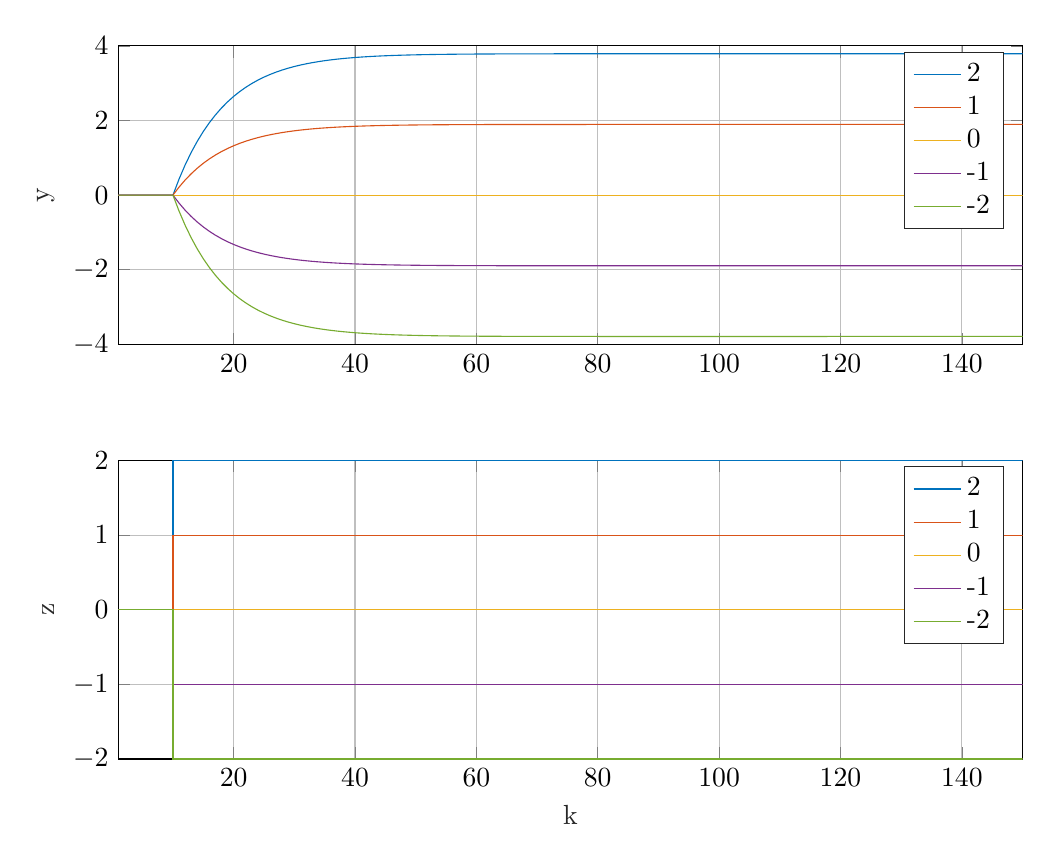
\begin{tikzpicture}

\begin{axis}[%
width=4.521in,
height=1.493in,
at={(0.758in,2.554in)},
scale only axis,
xmin=1,
xmax=150,
ymin=-4,
ymax=4,
ylabel style={font=\color{white!15!black}},
ylabel={y},
axis background/.style={fill=white},
xmajorgrids,
ymajorgrids,
legend style={legend cell align=left, align=left, draw=white!15!black}
]
\addplot [color=mycolor1]
  table[row sep=crcr]{%
1	0\\
2	0\\
3	0\\
4	0\\
5	0\\
6	0\\
7	0\\
8	0\\
9	0\\
10	0\\
11	0.4265\\
12	0.80513\\
13	1.1413\\
14	1.4396\\
15	1.7045\\
16	1.9396\\
17	2.1483\\
18	2.3336\\
19	2.498\\
20	2.6439\\
21	2.7734\\
22	2.8883\\
23	2.9903\\
24	3.0808\\
25	3.1611\\
26	3.2323\\
27	3.2955\\
28	3.3516\\
29	3.4013\\
30	3.4454\\
31	3.4846\\
32	3.5192\\
33	3.55\\
34	3.5773\\
35	3.6015\\
36	3.6229\\
37	3.6419\\
38	3.6587\\
39	3.6736\\
40	3.6868\\
41	3.6985\\
42	3.7089\\
43	3.7181\\
44	3.7262\\
45	3.7334\\
46	3.7398\\
47	3.7454\\
48	3.7504\\
49	3.7548\\
50	3.7586\\
51	3.7621\\
52	3.7651\\
53	3.7678\\
54	3.7702\\
55	3.7722\\
56	3.7741\\
57	3.7757\\
58	3.7771\\
59	3.7784\\
60	3.7795\\
61	3.7804\\
62	3.7813\\
63	3.782\\
64	3.7827\\
65	3.7833\\
66	3.7838\\
67	3.7842\\
68	3.7846\\
69	3.7849\\
70	3.7852\\
71	3.7855\\
72	3.7857\\
73	3.7859\\
74	3.786\\
75	3.7862\\
76	3.7863\\
77	3.7864\\
78	3.7865\\
79	3.7865\\
80	3.7866\\
81	3.7867\\
82	3.7867\\
83	3.7867\\
84	3.7868\\
85	3.7868\\
86	3.7868\\
87	3.7868\\
88	3.7868\\
89	3.7868\\
90	3.7868\\
91	3.7868\\
92	3.7868\\
93	3.7868\\
94	3.7868\\
95	3.7868\\
96	3.7868\\
97	3.7868\\
98	3.7868\\
99	3.7868\\
100	3.7868\\
101	3.7868\\
102	3.7868\\
103	3.7868\\
104	3.7867\\
105	3.7867\\
106	3.7867\\
107	3.7867\\
108	3.7867\\
109	3.7867\\
110	3.7867\\
111	3.7867\\
112	3.7867\\
113	3.7867\\
114	3.7867\\
115	3.7867\\
116	3.7867\\
117	3.7867\\
118	3.7866\\
119	3.7866\\
120	3.7866\\
121	3.7866\\
122	3.7866\\
123	3.7866\\
124	3.7866\\
125	3.7866\\
126	3.7866\\
127	3.7866\\
128	3.7866\\
129	3.7866\\
130	3.7866\\
131	3.7866\\
132	3.7866\\
133	3.7866\\
134	3.7866\\
135	3.7866\\
136	3.7866\\
137	3.7866\\
138	3.7866\\
139	3.7866\\
140	3.7866\\
141	3.7866\\
142	3.7866\\
143	3.7866\\
144	3.7866\\
145	3.7866\\
146	3.7866\\
147	3.7866\\
148	3.7866\\
149	3.7866\\
150	3.7866\\
151	3.7866\\
152	3.7866\\
153	3.7866\\
154	3.7866\\
155	3.7866\\
156	3.7865\\
157	3.7865\\
158	3.7865\\
159	3.7865\\
160	3.7865\\
161	3.7865\\
162	3.7865\\
163	3.7865\\
164	3.7865\\
165	3.7865\\
166	3.7865\\
167	3.7865\\
168	3.7865\\
169	3.7865\\
170	3.7865\\
171	3.7865\\
172	3.7865\\
173	3.7865\\
174	3.7865\\
175	3.7865\\
176	3.7865\\
177	3.7865\\
178	3.7865\\
179	3.7865\\
180	3.7865\\
181	3.7865\\
182	3.7865\\
183	3.7865\\
184	3.7865\\
185	3.7865\\
186	3.7865\\
187	3.7865\\
188	3.7865\\
189	3.7865\\
190	3.7865\\
191	3.7865\\
192	3.7865\\
193	3.7865\\
194	3.7865\\
195	3.7865\\
196	3.7865\\
197	3.7865\\
198	3.7865\\
199	3.7865\\
200	3.7865\\
201	3.7865\\
202	3.7865\\
203	3.7865\\
204	3.7865\\
205	3.7865\\
206	3.7865\\
207	3.7865\\
208	3.7865\\
209	3.7865\\
210	3.7865\\
211	3.7865\\
212	3.7865\\
213	3.7865\\
214	3.7865\\
215	3.7865\\
216	3.7865\\
217	3.7865\\
218	3.7865\\
219	3.7865\\
220	3.7865\\
221	3.7865\\
222	3.7865\\
223	3.7865\\
224	3.7865\\
225	3.7865\\
226	3.7865\\
227	3.7865\\
228	3.7865\\
229	3.7865\\
230	3.7865\\
231	3.7865\\
232	3.7865\\
233	3.7865\\
234	3.7865\\
235	3.7865\\
236	3.7865\\
237	3.7865\\
238	3.7865\\
239	3.7865\\
240	3.7865\\
241	3.7865\\
242	3.7865\\
243	3.7865\\
244	3.7865\\
245	3.7865\\
246	3.7865\\
247	3.7865\\
248	3.7865\\
249	3.7865\\
250	3.7865\\
251	3.7865\\
252	3.7865\\
253	3.7865\\
254	3.7865\\
255	3.7865\\
256	3.7865\\
257	3.7865\\
258	3.7865\\
259	3.7865\\
260	3.7865\\
261	3.7865\\
262	3.7865\\
263	3.7865\\
264	3.7865\\
265	3.7865\\
266	3.7865\\
267	3.7865\\
268	3.7865\\
269	3.7865\\
270	3.7865\\
271	3.7865\\
272	3.7865\\
273	3.7865\\
274	3.7865\\
275	3.7865\\
276	3.7865\\
277	3.7865\\
278	3.7865\\
279	3.7865\\
280	3.7865\\
281	3.7865\\
282	3.7865\\
283	3.7865\\
284	3.7865\\
285	3.7865\\
286	3.7865\\
287	3.7865\\
288	3.7865\\
289	3.7865\\
290	3.7865\\
291	3.7865\\
292	3.7865\\
293	3.7865\\
294	3.7865\\
295	3.7865\\
296	3.7865\\
297	3.7865\\
298	3.7865\\
299	3.7865\\
300	3.7865\\
};
\addlegendentry{2}

\addplot [color=mycolor2]
  table[row sep=crcr]{%
1	0\\
2	0\\
3	0\\
4	0\\
5	0\\
6	0\\
7	0\\
8	0\\
9	0\\
10	0\\
11	0.21325\\
12	0.40257\\
13	0.57063\\
14	0.71982\\
15	0.85226\\
16	0.96982\\
17	1.0742\\
18	1.1668\\
19	1.249\\
20	1.322\\
21	1.3867\\
22	1.4442\\
23	1.4952\\
24	1.5404\\
25	1.5805\\
26	1.6162\\
27	1.6478\\
28	1.6758\\
29	1.7007\\
30	1.7227\\
31	1.7423\\
32	1.7596\\
33	1.775\\
34	1.7886\\
35	1.8007\\
36	1.8114\\
37	1.8209\\
38	1.8294\\
39	1.8368\\
40	1.8434\\
41	1.8493\\
42	1.8545\\
43	1.859\\
44	1.8631\\
45	1.8667\\
46	1.8699\\
47	1.8727\\
48	1.8752\\
49	1.8774\\
50	1.8793\\
51	1.881\\
52	1.8826\\
53	1.8839\\
54	1.8851\\
55	1.8861\\
56	1.887\\
57	1.8878\\
58	1.8886\\
59	1.8892\\
60	1.8897\\
61	1.8902\\
62	1.8907\\
63	1.891\\
64	1.8914\\
65	1.8916\\
66	1.8919\\
67	1.8921\\
68	1.8923\\
69	1.8925\\
70	1.8926\\
71	1.8927\\
72	1.8928\\
73	1.8929\\
74	1.893\\
75	1.8931\\
76	1.8931\\
77	1.8932\\
78	1.8932\\
79	1.8933\\
80	1.8933\\
81	1.8933\\
82	1.8934\\
83	1.8934\\
84	1.8934\\
85	1.8934\\
86	1.8934\\
87	1.8934\\
88	1.8934\\
89	1.8934\\
90	1.8934\\
91	1.8934\\
92	1.8934\\
93	1.8934\\
94	1.8934\\
95	1.8934\\
96	1.8934\\
97	1.8934\\
98	1.8934\\
99	1.8934\\
100	1.8934\\
101	1.8934\\
102	1.8934\\
103	1.8934\\
104	1.8934\\
105	1.8934\\
106	1.8934\\
107	1.8934\\
108	1.8934\\
109	1.8934\\
110	1.8933\\
111	1.8933\\
112	1.8933\\
113	1.8933\\
114	1.8933\\
115	1.8933\\
116	1.8933\\
117	1.8933\\
118	1.8933\\
119	1.8933\\
120	1.8933\\
121	1.8933\\
122	1.8933\\
123	1.8933\\
124	1.8933\\
125	1.8933\\
126	1.8933\\
127	1.8933\\
128	1.8933\\
129	1.8933\\
130	1.8933\\
131	1.8933\\
132	1.8933\\
133	1.8933\\
134	1.8933\\
135	1.8933\\
136	1.8933\\
137	1.8933\\
138	1.8933\\
139	1.8933\\
140	1.8933\\
141	1.8933\\
142	1.8933\\
143	1.8933\\
144	1.8933\\
145	1.8933\\
146	1.8933\\
147	1.8933\\
148	1.8933\\
149	1.8933\\
150	1.8933\\
151	1.8933\\
152	1.8933\\
153	1.8933\\
154	1.8933\\
155	1.8933\\
156	1.8933\\
157	1.8933\\
158	1.8933\\
159	1.8933\\
160	1.8933\\
161	1.8933\\
162	1.8933\\
163	1.8933\\
164	1.8933\\
165	1.8933\\
166	1.8933\\
167	1.8933\\
168	1.8933\\
169	1.8933\\
170	1.8933\\
171	1.8933\\
172	1.8933\\
173	1.8933\\
174	1.8933\\
175	1.8933\\
176	1.8933\\
177	1.8933\\
178	1.8933\\
179	1.8933\\
180	1.8933\\
181	1.8933\\
182	1.8933\\
183	1.8933\\
184	1.8933\\
185	1.8933\\
186	1.8933\\
187	1.8933\\
188	1.8933\\
189	1.8933\\
190	1.8933\\
191	1.8933\\
192	1.8933\\
193	1.8933\\
194	1.8933\\
195	1.8933\\
196	1.8933\\
197	1.8933\\
198	1.8933\\
199	1.8933\\
200	1.8933\\
201	1.8933\\
202	1.8933\\
203	1.8933\\
204	1.8933\\
205	1.8933\\
206	1.8933\\
207	1.8933\\
208	1.8933\\
209	1.8933\\
210	1.8933\\
211	1.8933\\
212	1.8933\\
213	1.8933\\
214	1.8933\\
215	1.8933\\
216	1.8933\\
217	1.8933\\
218	1.8933\\
219	1.8933\\
220	1.8933\\
221	1.8933\\
222	1.8933\\
223	1.8933\\
224	1.8933\\
225	1.8933\\
226	1.8933\\
227	1.8933\\
228	1.8933\\
229	1.8933\\
230	1.8933\\
231	1.8933\\
232	1.8933\\
233	1.8933\\
234	1.8933\\
235	1.8933\\
236	1.8933\\
237	1.8933\\
238	1.8933\\
239	1.8933\\
240	1.8933\\
241	1.8933\\
242	1.8933\\
243	1.8933\\
244	1.8933\\
245	1.8933\\
246	1.8933\\
247	1.8933\\
248	1.8933\\
249	1.8933\\
250	1.8933\\
251	1.8933\\
252	1.8933\\
253	1.8933\\
254	1.8933\\
255	1.8933\\
256	1.8933\\
257	1.8933\\
258	1.8933\\
259	1.8933\\
260	1.8933\\
261	1.8933\\
262	1.8933\\
263	1.8933\\
264	1.8933\\
265	1.8933\\
266	1.8933\\
267	1.8933\\
268	1.8933\\
269	1.8933\\
270	1.8933\\
271	1.8933\\
272	1.8933\\
273	1.8933\\
274	1.8933\\
275	1.8933\\
276	1.8933\\
277	1.8933\\
278	1.8933\\
279	1.8933\\
280	1.8933\\
281	1.8933\\
282	1.8933\\
283	1.8933\\
284	1.8933\\
285	1.8933\\
286	1.8933\\
287	1.8933\\
288	1.8933\\
289	1.8933\\
290	1.8933\\
291	1.8933\\
292	1.8933\\
293	1.8933\\
294	1.8933\\
295	1.8933\\
296	1.8933\\
297	1.8933\\
298	1.8933\\
299	1.8933\\
300	1.8933\\
};
\addlegendentry{1}

\addplot [color=mycolor3]
  table[row sep=crcr]{%
1	0\\
2	0\\
3	0\\
4	0\\
5	0\\
6	0\\
7	0\\
8	0\\
9	0\\
10	0\\
11	0\\
12	0\\
13	0\\
14	0\\
15	0\\
16	0\\
17	0\\
18	0\\
19	0\\
20	0\\
21	0\\
22	0\\
23	0\\
24	0\\
25	0\\
26	0\\
27	0\\
28	0\\
29	0\\
30	0\\
31	0\\
32	0\\
33	0\\
34	0\\
35	0\\
36	0\\
37	0\\
38	0\\
39	0\\
40	0\\
41	0\\
42	0\\
43	0\\
44	0\\
45	0\\
46	0\\
47	0\\
48	0\\
49	0\\
50	0\\
51	0\\
52	0\\
53	0\\
54	0\\
55	0\\
56	0\\
57	0\\
58	0\\
59	0\\
60	0\\
61	0\\
62	0\\
63	0\\
64	0\\
65	0\\
66	0\\
67	0\\
68	0\\
69	0\\
70	0\\
71	0\\
72	0\\
73	0\\
74	0\\
75	0\\
76	0\\
77	0\\
78	0\\
79	0\\
80	0\\
81	0\\
82	0\\
83	0\\
84	0\\
85	0\\
86	0\\
87	0\\
88	0\\
89	0\\
90	0\\
91	0\\
92	0\\
93	0\\
94	0\\
95	0\\
96	0\\
97	0\\
98	0\\
99	0\\
100	0\\
101	0\\
102	0\\
103	0\\
104	0\\
105	0\\
106	0\\
107	0\\
108	0\\
109	0\\
110	0\\
111	0\\
112	0\\
113	0\\
114	0\\
115	0\\
116	0\\
117	0\\
118	0\\
119	0\\
120	0\\
121	0\\
122	0\\
123	0\\
124	0\\
125	0\\
126	0\\
127	0\\
128	0\\
129	0\\
130	0\\
131	0\\
132	0\\
133	0\\
134	0\\
135	0\\
136	0\\
137	0\\
138	0\\
139	0\\
140	0\\
141	0\\
142	0\\
143	0\\
144	0\\
145	0\\
146	0\\
147	0\\
148	0\\
149	0\\
150	0\\
151	0\\
152	0\\
153	0\\
154	0\\
155	0\\
156	0\\
157	0\\
158	0\\
159	0\\
160	0\\
161	0\\
162	0\\
163	0\\
164	0\\
165	0\\
166	0\\
167	0\\
168	0\\
169	0\\
170	0\\
171	0\\
172	0\\
173	0\\
174	0\\
175	0\\
176	0\\
177	0\\
178	0\\
179	0\\
180	0\\
181	0\\
182	0\\
183	0\\
184	0\\
185	0\\
186	0\\
187	0\\
188	0\\
189	0\\
190	0\\
191	0\\
192	0\\
193	0\\
194	0\\
195	0\\
196	0\\
197	0\\
198	0\\
199	0\\
200	0\\
201	0\\
202	0\\
203	0\\
204	0\\
205	0\\
206	0\\
207	0\\
208	0\\
209	0\\
210	0\\
211	0\\
212	0\\
213	0\\
214	0\\
215	0\\
216	0\\
217	0\\
218	0\\
219	0\\
220	0\\
221	0\\
222	0\\
223	0\\
224	0\\
225	0\\
226	0\\
227	0\\
228	0\\
229	0\\
230	0\\
231	0\\
232	0\\
233	0\\
234	0\\
235	0\\
236	0\\
237	0\\
238	0\\
239	0\\
240	0\\
241	0\\
242	0\\
243	0\\
244	0\\
245	0\\
246	0\\
247	0\\
248	0\\
249	0\\
250	0\\
251	0\\
252	0\\
253	0\\
254	0\\
255	0\\
256	0\\
257	0\\
258	0\\
259	0\\
260	0\\
261	0\\
262	0\\
263	0\\
264	0\\
265	0\\
266	0\\
267	0\\
268	0\\
269	0\\
270	0\\
271	0\\
272	0\\
273	0\\
274	0\\
275	0\\
276	0\\
277	0\\
278	0\\
279	0\\
280	0\\
281	0\\
282	0\\
283	0\\
284	0\\
285	0\\
286	0\\
287	0\\
288	0\\
289	0\\
290	0\\
291	0\\
292	0\\
293	0\\
294	0\\
295	0\\
296	0\\
297	0\\
298	0\\
299	0\\
300	0\\
};
\addlegendentry{0}

\addplot [color=mycolor4]
  table[row sep=crcr]{%
1	0\\
2	0\\
3	0\\
4	0\\
5	0\\
6	0\\
7	0\\
8	0\\
9	0\\
10	0\\
11	-0.21325\\
12	-0.40257\\
13	-0.57063\\
14	-0.71982\\
15	-0.85226\\
16	-0.96982\\
17	-1.0742\\
18	-1.1668\\
19	-1.249\\
20	-1.322\\
21	-1.3867\\
22	-1.4442\\
23	-1.4952\\
24	-1.5404\\
25	-1.5805\\
26	-1.6162\\
27	-1.6478\\
28	-1.6758\\
29	-1.7007\\
30	-1.7227\\
31	-1.7423\\
32	-1.7596\\
33	-1.775\\
34	-1.7886\\
35	-1.8007\\
36	-1.8114\\
37	-1.8209\\
38	-1.8294\\
39	-1.8368\\
40	-1.8434\\
41	-1.8493\\
42	-1.8545\\
43	-1.859\\
44	-1.8631\\
45	-1.8667\\
46	-1.8699\\
47	-1.8727\\
48	-1.8752\\
49	-1.8774\\
50	-1.8793\\
51	-1.881\\
52	-1.8826\\
53	-1.8839\\
54	-1.8851\\
55	-1.8861\\
56	-1.887\\
57	-1.8878\\
58	-1.8886\\
59	-1.8892\\
60	-1.8897\\
61	-1.8902\\
62	-1.8907\\
63	-1.891\\
64	-1.8914\\
65	-1.8916\\
66	-1.8919\\
67	-1.8921\\
68	-1.8923\\
69	-1.8925\\
70	-1.8926\\
71	-1.8927\\
72	-1.8928\\
73	-1.8929\\
74	-1.893\\
75	-1.8931\\
76	-1.8931\\
77	-1.8932\\
78	-1.8932\\
79	-1.8933\\
80	-1.8933\\
81	-1.8933\\
82	-1.8934\\
83	-1.8934\\
84	-1.8934\\
85	-1.8934\\
86	-1.8934\\
87	-1.8934\\
88	-1.8934\\
89	-1.8934\\
90	-1.8934\\
91	-1.8934\\
92	-1.8934\\
93	-1.8934\\
94	-1.8934\\
95	-1.8934\\
96	-1.8934\\
97	-1.8934\\
98	-1.8934\\
99	-1.8934\\
100	-1.8934\\
101	-1.8934\\
102	-1.8934\\
103	-1.8934\\
104	-1.8934\\
105	-1.8934\\
106	-1.8934\\
107	-1.8934\\
108	-1.8934\\
109	-1.8934\\
110	-1.8933\\
111	-1.8933\\
112	-1.8933\\
113	-1.8933\\
114	-1.8933\\
115	-1.8933\\
116	-1.8933\\
117	-1.8933\\
118	-1.8933\\
119	-1.8933\\
120	-1.8933\\
121	-1.8933\\
122	-1.8933\\
123	-1.8933\\
124	-1.8933\\
125	-1.8933\\
126	-1.8933\\
127	-1.8933\\
128	-1.8933\\
129	-1.8933\\
130	-1.8933\\
131	-1.8933\\
132	-1.8933\\
133	-1.8933\\
134	-1.8933\\
135	-1.8933\\
136	-1.8933\\
137	-1.8933\\
138	-1.8933\\
139	-1.8933\\
140	-1.8933\\
141	-1.8933\\
142	-1.8933\\
143	-1.8933\\
144	-1.8933\\
145	-1.8933\\
146	-1.8933\\
147	-1.8933\\
148	-1.8933\\
149	-1.8933\\
150	-1.8933\\
151	-1.8933\\
152	-1.8933\\
153	-1.8933\\
154	-1.8933\\
155	-1.8933\\
156	-1.8933\\
157	-1.8933\\
158	-1.8933\\
159	-1.8933\\
160	-1.8933\\
161	-1.8933\\
162	-1.8933\\
163	-1.8933\\
164	-1.8933\\
165	-1.8933\\
166	-1.8933\\
167	-1.8933\\
168	-1.8933\\
169	-1.8933\\
170	-1.8933\\
171	-1.8933\\
172	-1.8933\\
173	-1.8933\\
174	-1.8933\\
175	-1.8933\\
176	-1.8933\\
177	-1.8933\\
178	-1.8933\\
179	-1.8933\\
180	-1.8933\\
181	-1.8933\\
182	-1.8933\\
183	-1.8933\\
184	-1.8933\\
185	-1.8933\\
186	-1.8933\\
187	-1.8933\\
188	-1.8933\\
189	-1.8933\\
190	-1.8933\\
191	-1.8933\\
192	-1.8933\\
193	-1.8933\\
194	-1.8933\\
195	-1.8933\\
196	-1.8933\\
197	-1.8933\\
198	-1.8933\\
199	-1.8933\\
200	-1.8933\\
201	-1.8933\\
202	-1.8933\\
203	-1.8933\\
204	-1.8933\\
205	-1.8933\\
206	-1.8933\\
207	-1.8933\\
208	-1.8933\\
209	-1.8933\\
210	-1.8933\\
211	-1.8933\\
212	-1.8933\\
213	-1.8933\\
214	-1.8933\\
215	-1.8933\\
216	-1.8933\\
217	-1.8933\\
218	-1.8933\\
219	-1.8933\\
220	-1.8933\\
221	-1.8933\\
222	-1.8933\\
223	-1.8933\\
224	-1.8933\\
225	-1.8933\\
226	-1.8933\\
227	-1.8933\\
228	-1.8933\\
229	-1.8933\\
230	-1.8933\\
231	-1.8933\\
232	-1.8933\\
233	-1.8933\\
234	-1.8933\\
235	-1.8933\\
236	-1.8933\\
237	-1.8933\\
238	-1.8933\\
239	-1.8933\\
240	-1.8933\\
241	-1.8933\\
242	-1.8933\\
243	-1.8933\\
244	-1.8933\\
245	-1.8933\\
246	-1.8933\\
247	-1.8933\\
248	-1.8933\\
249	-1.8933\\
250	-1.8933\\
251	-1.8933\\
252	-1.8933\\
253	-1.8933\\
254	-1.8933\\
255	-1.8933\\
256	-1.8933\\
257	-1.8933\\
258	-1.8933\\
259	-1.8933\\
260	-1.8933\\
261	-1.8933\\
262	-1.8933\\
263	-1.8933\\
264	-1.8933\\
265	-1.8933\\
266	-1.8933\\
267	-1.8933\\
268	-1.8933\\
269	-1.8933\\
270	-1.8933\\
271	-1.8933\\
272	-1.8933\\
273	-1.8933\\
274	-1.8933\\
275	-1.8933\\
276	-1.8933\\
277	-1.8933\\
278	-1.8933\\
279	-1.8933\\
280	-1.8933\\
281	-1.8933\\
282	-1.8933\\
283	-1.8933\\
284	-1.8933\\
285	-1.8933\\
286	-1.8933\\
287	-1.8933\\
288	-1.8933\\
289	-1.8933\\
290	-1.8933\\
291	-1.8933\\
292	-1.8933\\
293	-1.8933\\
294	-1.8933\\
295	-1.8933\\
296	-1.8933\\
297	-1.8933\\
298	-1.8933\\
299	-1.8933\\
300	-1.8933\\
};
\addlegendentry{-1}

\addplot [color=mycolor5]
  table[row sep=crcr]{%
1	0\\
2	0\\
3	0\\
4	0\\
5	0\\
6	0\\
7	0\\
8	0\\
9	0\\
10	0\\
11	-0.4265\\
12	-0.80513\\
13	-1.1413\\
14	-1.4396\\
15	-1.7045\\
16	-1.9396\\
17	-2.1483\\
18	-2.3336\\
19	-2.498\\
20	-2.6439\\
21	-2.7734\\
22	-2.8883\\
23	-2.9903\\
24	-3.0808\\
25	-3.1611\\
26	-3.2323\\
27	-3.2955\\
28	-3.3516\\
29	-3.4013\\
30	-3.4454\\
31	-3.4846\\
32	-3.5192\\
33	-3.55\\
34	-3.5773\\
35	-3.6015\\
36	-3.6229\\
37	-3.6419\\
38	-3.6587\\
39	-3.6736\\
40	-3.6868\\
41	-3.6985\\
42	-3.7089\\
43	-3.7181\\
44	-3.7262\\
45	-3.7334\\
46	-3.7398\\
47	-3.7454\\
48	-3.7504\\
49	-3.7548\\
50	-3.7586\\
51	-3.7621\\
52	-3.7651\\
53	-3.7678\\
54	-3.7702\\
55	-3.7722\\
56	-3.7741\\
57	-3.7757\\
58	-3.7771\\
59	-3.7784\\
60	-3.7795\\
61	-3.7804\\
62	-3.7813\\
63	-3.782\\
64	-3.7827\\
65	-3.7833\\
66	-3.7838\\
67	-3.7842\\
68	-3.7846\\
69	-3.7849\\
70	-3.7852\\
71	-3.7855\\
72	-3.7857\\
73	-3.7859\\
74	-3.786\\
75	-3.7862\\
76	-3.7863\\
77	-3.7864\\
78	-3.7865\\
79	-3.7865\\
80	-3.7866\\
81	-3.7867\\
82	-3.7867\\
83	-3.7867\\
84	-3.7868\\
85	-3.7868\\
86	-3.7868\\
87	-3.7868\\
88	-3.7868\\
89	-3.7868\\
90	-3.7868\\
91	-3.7868\\
92	-3.7868\\
93	-3.7868\\
94	-3.7868\\
95	-3.7868\\
96	-3.7868\\
97	-3.7868\\
98	-3.7868\\
99	-3.7868\\
100	-3.7868\\
101	-3.7868\\
102	-3.7868\\
103	-3.7868\\
104	-3.7867\\
105	-3.7867\\
106	-3.7867\\
107	-3.7867\\
108	-3.7867\\
109	-3.7867\\
110	-3.7867\\
111	-3.7867\\
112	-3.7867\\
113	-3.7867\\
114	-3.7867\\
115	-3.7867\\
116	-3.7867\\
117	-3.7867\\
118	-3.7866\\
119	-3.7866\\
120	-3.7866\\
121	-3.7866\\
122	-3.7866\\
123	-3.7866\\
124	-3.7866\\
125	-3.7866\\
126	-3.7866\\
127	-3.7866\\
128	-3.7866\\
129	-3.7866\\
130	-3.7866\\
131	-3.7866\\
132	-3.7866\\
133	-3.7866\\
134	-3.7866\\
135	-3.7866\\
136	-3.7866\\
137	-3.7866\\
138	-3.7866\\
139	-3.7866\\
140	-3.7866\\
141	-3.7866\\
142	-3.7866\\
143	-3.7866\\
144	-3.7866\\
145	-3.7866\\
146	-3.7866\\
147	-3.7866\\
148	-3.7866\\
149	-3.7866\\
150	-3.7866\\
151	-3.7866\\
152	-3.7866\\
153	-3.7866\\
154	-3.7866\\
155	-3.7866\\
156	-3.7865\\
157	-3.7865\\
158	-3.7865\\
159	-3.7865\\
160	-3.7865\\
161	-3.7865\\
162	-3.7865\\
163	-3.7865\\
164	-3.7865\\
165	-3.7865\\
166	-3.7865\\
167	-3.7865\\
168	-3.7865\\
169	-3.7865\\
170	-3.7865\\
171	-3.7865\\
172	-3.7865\\
173	-3.7865\\
174	-3.7865\\
175	-3.7865\\
176	-3.7865\\
177	-3.7865\\
178	-3.7865\\
179	-3.7865\\
180	-3.7865\\
181	-3.7865\\
182	-3.7865\\
183	-3.7865\\
184	-3.7865\\
185	-3.7865\\
186	-3.7865\\
187	-3.7865\\
188	-3.7865\\
189	-3.7865\\
190	-3.7865\\
191	-3.7865\\
192	-3.7865\\
193	-3.7865\\
194	-3.7865\\
195	-3.7865\\
196	-3.7865\\
197	-3.7865\\
198	-3.7865\\
199	-3.7865\\
200	-3.7865\\
201	-3.7865\\
202	-3.7865\\
203	-3.7865\\
204	-3.7865\\
205	-3.7865\\
206	-3.7865\\
207	-3.7865\\
208	-3.7865\\
209	-3.7865\\
210	-3.7865\\
211	-3.7865\\
212	-3.7865\\
213	-3.7865\\
214	-3.7865\\
215	-3.7865\\
216	-3.7865\\
217	-3.7865\\
218	-3.7865\\
219	-3.7865\\
220	-3.7865\\
221	-3.7865\\
222	-3.7865\\
223	-3.7865\\
224	-3.7865\\
225	-3.7865\\
226	-3.7865\\
227	-3.7865\\
228	-3.7865\\
229	-3.7865\\
230	-3.7865\\
231	-3.7865\\
232	-3.7865\\
233	-3.7865\\
234	-3.7865\\
235	-3.7865\\
236	-3.7865\\
237	-3.7865\\
238	-3.7865\\
239	-3.7865\\
240	-3.7865\\
241	-3.7865\\
242	-3.7865\\
243	-3.7865\\
244	-3.7865\\
245	-3.7865\\
246	-3.7865\\
247	-3.7865\\
248	-3.7865\\
249	-3.7865\\
250	-3.7865\\
251	-3.7865\\
252	-3.7865\\
253	-3.7865\\
254	-3.7865\\
255	-3.7865\\
256	-3.7865\\
257	-3.7865\\
258	-3.7865\\
259	-3.7865\\
260	-3.7865\\
261	-3.7865\\
262	-3.7865\\
263	-3.7865\\
264	-3.7865\\
265	-3.7865\\
266	-3.7865\\
267	-3.7865\\
268	-3.7865\\
269	-3.7865\\
270	-3.7865\\
271	-3.7865\\
272	-3.7865\\
273	-3.7865\\
274	-3.7865\\
275	-3.7865\\
276	-3.7865\\
277	-3.7865\\
278	-3.7865\\
279	-3.7865\\
280	-3.7865\\
281	-3.7865\\
282	-3.7865\\
283	-3.7865\\
284	-3.7865\\
285	-3.7865\\
286	-3.7865\\
287	-3.7865\\
288	-3.7865\\
289	-3.7865\\
290	-3.7865\\
291	-3.7865\\
292	-3.7865\\
293	-3.7865\\
294	-3.7865\\
295	-3.7865\\
296	-3.7865\\
297	-3.7865\\
298	-3.7865\\
299	-3.7865\\
300	-3.7865\\
};
\addlegendentry{-2}

\end{axis}

\begin{axis}[%
width=4.521in,
height=1.493in,
at={(0.758in,0.481in)},
scale only axis,
xmin=1,
xmax=150,
xlabel style={font=\color{white!15!black}},
xlabel={k},
ymin=-2,
ymax=2,
ylabel style={font=\color{white!15!black}},
ylabel={z},
axis background/.style={fill=white},
xmajorgrids,
ymajorgrids,
legend style={legend cell align=left, align=left, draw=white!15!black}
]
\addplot[const plot, color=mycolor1] table[row sep=crcr] {%
1	0\\
2	0\\
3	0\\
4	0\\
5	0\\
6	0\\
7	0\\
8	0\\
9	0\\
10	2\\
11	2\\
12	2\\
13	2\\
14	2\\
15	2\\
16	2\\
17	2\\
18	2\\
19	2\\
20	2\\
21	2\\
22	2\\
23	2\\
24	2\\
25	2\\
26	2\\
27	2\\
28	2\\
29	2\\
30	2\\
31	2\\
32	2\\
33	2\\
34	2\\
35	2\\
36	2\\
37	2\\
38	2\\
39	2\\
40	2\\
41	2\\
42	2\\
43	2\\
44	2\\
45	2\\
46	2\\
47	2\\
48	2\\
49	2\\
50	2\\
51	2\\
52	2\\
53	2\\
54	2\\
55	2\\
56	2\\
57	2\\
58	2\\
59	2\\
60	2\\
61	2\\
62	2\\
63	2\\
64	2\\
65	2\\
66	2\\
67	2\\
68	2\\
69	2\\
70	2\\
71	2\\
72	2\\
73	2\\
74	2\\
75	2\\
76	2\\
77	2\\
78	2\\
79	2\\
80	2\\
81	2\\
82	2\\
83	2\\
84	2\\
85	2\\
86	2\\
87	2\\
88	2\\
89	2\\
90	2\\
91	2\\
92	2\\
93	2\\
94	2\\
95	2\\
96	2\\
97	2\\
98	2\\
99	2\\
100	2\\
101	2\\
102	2\\
103	2\\
104	2\\
105	2\\
106	2\\
107	2\\
108	2\\
109	2\\
110	2\\
111	2\\
112	2\\
113	2\\
114	2\\
115	2\\
116	2\\
117	2\\
118	2\\
119	2\\
120	2\\
121	2\\
122	2\\
123	2\\
124	2\\
125	2\\
126	2\\
127	2\\
128	2\\
129	2\\
130	2\\
131	2\\
132	2\\
133	2\\
134	2\\
135	2\\
136	2\\
137	2\\
138	2\\
139	2\\
140	2\\
141	2\\
142	2\\
143	2\\
144	2\\
145	2\\
146	2\\
147	2\\
148	2\\
149	2\\
150	2\\
151	2\\
152	2\\
153	2\\
154	2\\
155	2\\
156	2\\
157	2\\
158	2\\
159	2\\
160	2\\
161	2\\
162	2\\
163	2\\
164	2\\
165	2\\
166	2\\
167	2\\
168	2\\
169	2\\
170	2\\
171	2\\
172	2\\
173	2\\
174	2\\
175	2\\
176	2\\
177	2\\
178	2\\
179	2\\
180	2\\
181	2\\
182	2\\
183	2\\
184	2\\
185	2\\
186	2\\
187	2\\
188	2\\
189	2\\
190	2\\
191	2\\
192	2\\
193	2\\
194	2\\
195	2\\
196	2\\
197	2\\
198	2\\
199	2\\
200	2\\
201	2\\
202	2\\
203	2\\
204	2\\
205	2\\
206	2\\
207	2\\
208	2\\
209	2\\
210	2\\
211	2\\
212	2\\
213	2\\
214	2\\
215	2\\
216	2\\
217	2\\
218	2\\
219	2\\
220	2\\
221	2\\
222	2\\
223	2\\
224	2\\
225	2\\
226	2\\
227	2\\
228	2\\
229	2\\
230	2\\
231	2\\
232	2\\
233	2\\
234	2\\
235	2\\
236	2\\
237	2\\
238	2\\
239	2\\
240	2\\
241	2\\
242	2\\
243	2\\
244	2\\
245	2\\
246	2\\
247	2\\
248	2\\
249	2\\
250	2\\
251	2\\
252	2\\
253	2\\
254	2\\
255	2\\
256	2\\
257	2\\
258	2\\
259	2\\
260	2\\
261	2\\
262	2\\
263	2\\
264	2\\
265	2\\
266	2\\
267	2\\
268	2\\
269	2\\
270	2\\
271	2\\
272	2\\
273	2\\
274	2\\
275	2\\
276	2\\
277	2\\
278	2\\
279	2\\
280	2\\
281	2\\
282	2\\
283	2\\
284	2\\
285	2\\
286	2\\
287	2\\
288	2\\
289	2\\
290	2\\
291	2\\
292	2\\
293	2\\
294	2\\
295	2\\
296	2\\
297	2\\
298	2\\
299	2\\
300	2\\
};
\addlegendentry{2}

\addplot[const plot, color=mycolor2] table[row sep=crcr] {%
1	0\\
2	0\\
3	0\\
4	0\\
5	0\\
6	0\\
7	0\\
8	0\\
9	0\\
10	1\\
11	1\\
12	1\\
13	1\\
14	1\\
15	1\\
16	1\\
17	1\\
18	1\\
19	1\\
20	1\\
21	1\\
22	1\\
23	1\\
24	1\\
25	1\\
26	1\\
27	1\\
28	1\\
29	1\\
30	1\\
31	1\\
32	1\\
33	1\\
34	1\\
35	1\\
36	1\\
37	1\\
38	1\\
39	1\\
40	1\\
41	1\\
42	1\\
43	1\\
44	1\\
45	1\\
46	1\\
47	1\\
48	1\\
49	1\\
50	1\\
51	1\\
52	1\\
53	1\\
54	1\\
55	1\\
56	1\\
57	1\\
58	1\\
59	1\\
60	1\\
61	1\\
62	1\\
63	1\\
64	1\\
65	1\\
66	1\\
67	1\\
68	1\\
69	1\\
70	1\\
71	1\\
72	1\\
73	1\\
74	1\\
75	1\\
76	1\\
77	1\\
78	1\\
79	1\\
80	1\\
81	1\\
82	1\\
83	1\\
84	1\\
85	1\\
86	1\\
87	1\\
88	1\\
89	1\\
90	1\\
91	1\\
92	1\\
93	1\\
94	1\\
95	1\\
96	1\\
97	1\\
98	1\\
99	1\\
100	1\\
101	1\\
102	1\\
103	1\\
104	1\\
105	1\\
106	1\\
107	1\\
108	1\\
109	1\\
110	1\\
111	1\\
112	1\\
113	1\\
114	1\\
115	1\\
116	1\\
117	1\\
118	1\\
119	1\\
120	1\\
121	1\\
122	1\\
123	1\\
124	1\\
125	1\\
126	1\\
127	1\\
128	1\\
129	1\\
130	1\\
131	1\\
132	1\\
133	1\\
134	1\\
135	1\\
136	1\\
137	1\\
138	1\\
139	1\\
140	1\\
141	1\\
142	1\\
143	1\\
144	1\\
145	1\\
146	1\\
147	1\\
148	1\\
149	1\\
150	1\\
151	1\\
152	1\\
153	1\\
154	1\\
155	1\\
156	1\\
157	1\\
158	1\\
159	1\\
160	1\\
161	1\\
162	1\\
163	1\\
164	1\\
165	1\\
166	1\\
167	1\\
168	1\\
169	1\\
170	1\\
171	1\\
172	1\\
173	1\\
174	1\\
175	1\\
176	1\\
177	1\\
178	1\\
179	1\\
180	1\\
181	1\\
182	1\\
183	1\\
184	1\\
185	1\\
186	1\\
187	1\\
188	1\\
189	1\\
190	1\\
191	1\\
192	1\\
193	1\\
194	1\\
195	1\\
196	1\\
197	1\\
198	1\\
199	1\\
200	1\\
201	1\\
202	1\\
203	1\\
204	1\\
205	1\\
206	1\\
207	1\\
208	1\\
209	1\\
210	1\\
211	1\\
212	1\\
213	1\\
214	1\\
215	1\\
216	1\\
217	1\\
218	1\\
219	1\\
220	1\\
221	1\\
222	1\\
223	1\\
224	1\\
225	1\\
226	1\\
227	1\\
228	1\\
229	1\\
230	1\\
231	1\\
232	1\\
233	1\\
234	1\\
235	1\\
236	1\\
237	1\\
238	1\\
239	1\\
240	1\\
241	1\\
242	1\\
243	1\\
244	1\\
245	1\\
246	1\\
247	1\\
248	1\\
249	1\\
250	1\\
251	1\\
252	1\\
253	1\\
254	1\\
255	1\\
256	1\\
257	1\\
258	1\\
259	1\\
260	1\\
261	1\\
262	1\\
263	1\\
264	1\\
265	1\\
266	1\\
267	1\\
268	1\\
269	1\\
270	1\\
271	1\\
272	1\\
273	1\\
274	1\\
275	1\\
276	1\\
277	1\\
278	1\\
279	1\\
280	1\\
281	1\\
282	1\\
283	1\\
284	1\\
285	1\\
286	1\\
287	1\\
288	1\\
289	1\\
290	1\\
291	1\\
292	1\\
293	1\\
294	1\\
295	1\\
296	1\\
297	1\\
298	1\\
299	1\\
300	1\\
};
\addlegendentry{1}

\addplot[const plot, color=mycolor3] table[row sep=crcr] {%
1	0\\
2	0\\
3	0\\
4	0\\
5	0\\
6	0\\
7	0\\
8	0\\
9	0\\
10	0\\
11	0\\
12	0\\
13	0\\
14	0\\
15	0\\
16	0\\
17	0\\
18	0\\
19	0\\
20	0\\
21	0\\
22	0\\
23	0\\
24	0\\
25	0\\
26	0\\
27	0\\
28	0\\
29	0\\
30	0\\
31	0\\
32	0\\
33	0\\
34	0\\
35	0\\
36	0\\
37	0\\
38	0\\
39	0\\
40	0\\
41	0\\
42	0\\
43	0\\
44	0\\
45	0\\
46	0\\
47	0\\
48	0\\
49	0\\
50	0\\
51	0\\
52	0\\
53	0\\
54	0\\
55	0\\
56	0\\
57	0\\
58	0\\
59	0\\
60	0\\
61	0\\
62	0\\
63	0\\
64	0\\
65	0\\
66	0\\
67	0\\
68	0\\
69	0\\
70	0\\
71	0\\
72	0\\
73	0\\
74	0\\
75	0\\
76	0\\
77	0\\
78	0\\
79	0\\
80	0\\
81	0\\
82	0\\
83	0\\
84	0\\
85	0\\
86	0\\
87	0\\
88	0\\
89	0\\
90	0\\
91	0\\
92	0\\
93	0\\
94	0\\
95	0\\
96	0\\
97	0\\
98	0\\
99	0\\
100	0\\
101	0\\
102	0\\
103	0\\
104	0\\
105	0\\
106	0\\
107	0\\
108	0\\
109	0\\
110	0\\
111	0\\
112	0\\
113	0\\
114	0\\
115	0\\
116	0\\
117	0\\
118	0\\
119	0\\
120	0\\
121	0\\
122	0\\
123	0\\
124	0\\
125	0\\
126	0\\
127	0\\
128	0\\
129	0\\
130	0\\
131	0\\
132	0\\
133	0\\
134	0\\
135	0\\
136	0\\
137	0\\
138	0\\
139	0\\
140	0\\
141	0\\
142	0\\
143	0\\
144	0\\
145	0\\
146	0\\
147	0\\
148	0\\
149	0\\
150	0\\
151	0\\
152	0\\
153	0\\
154	0\\
155	0\\
156	0\\
157	0\\
158	0\\
159	0\\
160	0\\
161	0\\
162	0\\
163	0\\
164	0\\
165	0\\
166	0\\
167	0\\
168	0\\
169	0\\
170	0\\
171	0\\
172	0\\
173	0\\
174	0\\
175	0\\
176	0\\
177	0\\
178	0\\
179	0\\
180	0\\
181	0\\
182	0\\
183	0\\
184	0\\
185	0\\
186	0\\
187	0\\
188	0\\
189	0\\
190	0\\
191	0\\
192	0\\
193	0\\
194	0\\
195	0\\
196	0\\
197	0\\
198	0\\
199	0\\
200	0\\
201	0\\
202	0\\
203	0\\
204	0\\
205	0\\
206	0\\
207	0\\
208	0\\
209	0\\
210	0\\
211	0\\
212	0\\
213	0\\
214	0\\
215	0\\
216	0\\
217	0\\
218	0\\
219	0\\
220	0\\
221	0\\
222	0\\
223	0\\
224	0\\
225	0\\
226	0\\
227	0\\
228	0\\
229	0\\
230	0\\
231	0\\
232	0\\
233	0\\
234	0\\
235	0\\
236	0\\
237	0\\
238	0\\
239	0\\
240	0\\
241	0\\
242	0\\
243	0\\
244	0\\
245	0\\
246	0\\
247	0\\
248	0\\
249	0\\
250	0\\
251	0\\
252	0\\
253	0\\
254	0\\
255	0\\
256	0\\
257	0\\
258	0\\
259	0\\
260	0\\
261	0\\
262	0\\
263	0\\
264	0\\
265	0\\
266	0\\
267	0\\
268	0\\
269	0\\
270	0\\
271	0\\
272	0\\
273	0\\
274	0\\
275	0\\
276	0\\
277	0\\
278	0\\
279	0\\
280	0\\
281	0\\
282	0\\
283	0\\
284	0\\
285	0\\
286	0\\
287	0\\
288	0\\
289	0\\
290	0\\
291	0\\
292	0\\
293	0\\
294	0\\
295	0\\
296	0\\
297	0\\
298	0\\
299	0\\
300	0\\
};
\addlegendentry{0}

\addplot[const plot, color=mycolor4] table[row sep=crcr] {%
1	0\\
2	0\\
3	0\\
4	0\\
5	0\\
6	0\\
7	0\\
8	0\\
9	0\\
10	-1\\
11	-1\\
12	-1\\
13	-1\\
14	-1\\
15	-1\\
16	-1\\
17	-1\\
18	-1\\
19	-1\\
20	-1\\
21	-1\\
22	-1\\
23	-1\\
24	-1\\
25	-1\\
26	-1\\
27	-1\\
28	-1\\
29	-1\\
30	-1\\
31	-1\\
32	-1\\
33	-1\\
34	-1\\
35	-1\\
36	-1\\
37	-1\\
38	-1\\
39	-1\\
40	-1\\
41	-1\\
42	-1\\
43	-1\\
44	-1\\
45	-1\\
46	-1\\
47	-1\\
48	-1\\
49	-1\\
50	-1\\
51	-1\\
52	-1\\
53	-1\\
54	-1\\
55	-1\\
56	-1\\
57	-1\\
58	-1\\
59	-1\\
60	-1\\
61	-1\\
62	-1\\
63	-1\\
64	-1\\
65	-1\\
66	-1\\
67	-1\\
68	-1\\
69	-1\\
70	-1\\
71	-1\\
72	-1\\
73	-1\\
74	-1\\
75	-1\\
76	-1\\
77	-1\\
78	-1\\
79	-1\\
80	-1\\
81	-1\\
82	-1\\
83	-1\\
84	-1\\
85	-1\\
86	-1\\
87	-1\\
88	-1\\
89	-1\\
90	-1\\
91	-1\\
92	-1\\
93	-1\\
94	-1\\
95	-1\\
96	-1\\
97	-1\\
98	-1\\
99	-1\\
100	-1\\
101	-1\\
102	-1\\
103	-1\\
104	-1\\
105	-1\\
106	-1\\
107	-1\\
108	-1\\
109	-1\\
110	-1\\
111	-1\\
112	-1\\
113	-1\\
114	-1\\
115	-1\\
116	-1\\
117	-1\\
118	-1\\
119	-1\\
120	-1\\
121	-1\\
122	-1\\
123	-1\\
124	-1\\
125	-1\\
126	-1\\
127	-1\\
128	-1\\
129	-1\\
130	-1\\
131	-1\\
132	-1\\
133	-1\\
134	-1\\
135	-1\\
136	-1\\
137	-1\\
138	-1\\
139	-1\\
140	-1\\
141	-1\\
142	-1\\
143	-1\\
144	-1\\
145	-1\\
146	-1\\
147	-1\\
148	-1\\
149	-1\\
150	-1\\
151	-1\\
152	-1\\
153	-1\\
154	-1\\
155	-1\\
156	-1\\
157	-1\\
158	-1\\
159	-1\\
160	-1\\
161	-1\\
162	-1\\
163	-1\\
164	-1\\
165	-1\\
166	-1\\
167	-1\\
168	-1\\
169	-1\\
170	-1\\
171	-1\\
172	-1\\
173	-1\\
174	-1\\
175	-1\\
176	-1\\
177	-1\\
178	-1\\
179	-1\\
180	-1\\
181	-1\\
182	-1\\
183	-1\\
184	-1\\
185	-1\\
186	-1\\
187	-1\\
188	-1\\
189	-1\\
190	-1\\
191	-1\\
192	-1\\
193	-1\\
194	-1\\
195	-1\\
196	-1\\
197	-1\\
198	-1\\
199	-1\\
200	-1\\
201	-1\\
202	-1\\
203	-1\\
204	-1\\
205	-1\\
206	-1\\
207	-1\\
208	-1\\
209	-1\\
210	-1\\
211	-1\\
212	-1\\
213	-1\\
214	-1\\
215	-1\\
216	-1\\
217	-1\\
218	-1\\
219	-1\\
220	-1\\
221	-1\\
222	-1\\
223	-1\\
224	-1\\
225	-1\\
226	-1\\
227	-1\\
228	-1\\
229	-1\\
230	-1\\
231	-1\\
232	-1\\
233	-1\\
234	-1\\
235	-1\\
236	-1\\
237	-1\\
238	-1\\
239	-1\\
240	-1\\
241	-1\\
242	-1\\
243	-1\\
244	-1\\
245	-1\\
246	-1\\
247	-1\\
248	-1\\
249	-1\\
250	-1\\
251	-1\\
252	-1\\
253	-1\\
254	-1\\
255	-1\\
256	-1\\
257	-1\\
258	-1\\
259	-1\\
260	-1\\
261	-1\\
262	-1\\
263	-1\\
264	-1\\
265	-1\\
266	-1\\
267	-1\\
268	-1\\
269	-1\\
270	-1\\
271	-1\\
272	-1\\
273	-1\\
274	-1\\
275	-1\\
276	-1\\
277	-1\\
278	-1\\
279	-1\\
280	-1\\
281	-1\\
282	-1\\
283	-1\\
284	-1\\
285	-1\\
286	-1\\
287	-1\\
288	-1\\
289	-1\\
290	-1\\
291	-1\\
292	-1\\
293	-1\\
294	-1\\
295	-1\\
296	-1\\
297	-1\\
298	-1\\
299	-1\\
300	-1\\
};
\addlegendentry{-1}

\addplot[const plot, color=mycolor5] table[row sep=crcr] {%
1	0\\
2	0\\
3	0\\
4	0\\
5	0\\
6	0\\
7	0\\
8	0\\
9	0\\
10	-2\\
11	-2\\
12	-2\\
13	-2\\
14	-2\\
15	-2\\
16	-2\\
17	-2\\
18	-2\\
19	-2\\
20	-2\\
21	-2\\
22	-2\\
23	-2\\
24	-2\\
25	-2\\
26	-2\\
27	-2\\
28	-2\\
29	-2\\
30	-2\\
31	-2\\
32	-2\\
33	-2\\
34	-2\\
35	-2\\
36	-2\\
37	-2\\
38	-2\\
39	-2\\
40	-2\\
41	-2\\
42	-2\\
43	-2\\
44	-2\\
45	-2\\
46	-2\\
47	-2\\
48	-2\\
49	-2\\
50	-2\\
51	-2\\
52	-2\\
53	-2\\
54	-2\\
55	-2\\
56	-2\\
57	-2\\
58	-2\\
59	-2\\
60	-2\\
61	-2\\
62	-2\\
63	-2\\
64	-2\\
65	-2\\
66	-2\\
67	-2\\
68	-2\\
69	-2\\
70	-2\\
71	-2\\
72	-2\\
73	-2\\
74	-2\\
75	-2\\
76	-2\\
77	-2\\
78	-2\\
79	-2\\
80	-2\\
81	-2\\
82	-2\\
83	-2\\
84	-2\\
85	-2\\
86	-2\\
87	-2\\
88	-2\\
89	-2\\
90	-2\\
91	-2\\
92	-2\\
93	-2\\
94	-2\\
95	-2\\
96	-2\\
97	-2\\
98	-2\\
99	-2\\
100	-2\\
101	-2\\
102	-2\\
103	-2\\
104	-2\\
105	-2\\
106	-2\\
107	-2\\
108	-2\\
109	-2\\
110	-2\\
111	-2\\
112	-2\\
113	-2\\
114	-2\\
115	-2\\
116	-2\\
117	-2\\
118	-2\\
119	-2\\
120	-2\\
121	-2\\
122	-2\\
123	-2\\
124	-2\\
125	-2\\
126	-2\\
127	-2\\
128	-2\\
129	-2\\
130	-2\\
131	-2\\
132	-2\\
133	-2\\
134	-2\\
135	-2\\
136	-2\\
137	-2\\
138	-2\\
139	-2\\
140	-2\\
141	-2\\
142	-2\\
143	-2\\
144	-2\\
145	-2\\
146	-2\\
147	-2\\
148	-2\\
149	-2\\
150	-2\\
151	-2\\
152	-2\\
153	-2\\
154	-2\\
155	-2\\
156	-2\\
157	-2\\
158	-2\\
159	-2\\
160	-2\\
161	-2\\
162	-2\\
163	-2\\
164	-2\\
165	-2\\
166	-2\\
167	-2\\
168	-2\\
169	-2\\
170	-2\\
171	-2\\
172	-2\\
173	-2\\
174	-2\\
175	-2\\
176	-2\\
177	-2\\
178	-2\\
179	-2\\
180	-2\\
181	-2\\
182	-2\\
183	-2\\
184	-2\\
185	-2\\
186	-2\\
187	-2\\
188	-2\\
189	-2\\
190	-2\\
191	-2\\
192	-2\\
193	-2\\
194	-2\\
195	-2\\
196	-2\\
197	-2\\
198	-2\\
199	-2\\
200	-2\\
201	-2\\
202	-2\\
203	-2\\
204	-2\\
205	-2\\
206	-2\\
207	-2\\
208	-2\\
209	-2\\
210	-2\\
211	-2\\
212	-2\\
213	-2\\
214	-2\\
215	-2\\
216	-2\\
217	-2\\
218	-2\\
219	-2\\
220	-2\\
221	-2\\
222	-2\\
223	-2\\
224	-2\\
225	-2\\
226	-2\\
227	-2\\
228	-2\\
229	-2\\
230	-2\\
231	-2\\
232	-2\\
233	-2\\
234	-2\\
235	-2\\
236	-2\\
237	-2\\
238	-2\\
239	-2\\
240	-2\\
241	-2\\
242	-2\\
243	-2\\
244	-2\\
245	-2\\
246	-2\\
247	-2\\
248	-2\\
249	-2\\
250	-2\\
251	-2\\
252	-2\\
253	-2\\
254	-2\\
255	-2\\
256	-2\\
257	-2\\
258	-2\\
259	-2\\
260	-2\\
261	-2\\
262	-2\\
263	-2\\
264	-2\\
265	-2\\
266	-2\\
267	-2\\
268	-2\\
269	-2\\
270	-2\\
271	-2\\
272	-2\\
273	-2\\
274	-2\\
275	-2\\
276	-2\\
277	-2\\
278	-2\\
279	-2\\
280	-2\\
281	-2\\
282	-2\\
283	-2\\
284	-2\\
285	-2\\
286	-2\\
287	-2\\
288	-2\\
289	-2\\
290	-2\\
291	-2\\
292	-2\\
293	-2\\
294	-2\\
295	-2\\
296	-2\\
297	-2\\
298	-2\\
299	-2\\
300	-2\\
};
\addlegendentry{-2}

\end{axis}
\end{tikzpicture}%
    \caption{Odpowiedzi skokowe obiektu od zakłócenia}
    \label{projekt:zad2:StepYZ:figure}
\end{figure}

\subsection{Charakterystyka statyczna Y(U, Z)}
\label{projekt:zad2:charStat}

Dzięki uzyskanym odpowiedziom skokowym otrzymano charakterystykę statyczną y(u,z)

\begin{figure}[H] 
    \centering
    % This file was created by matlab2tikz.
%
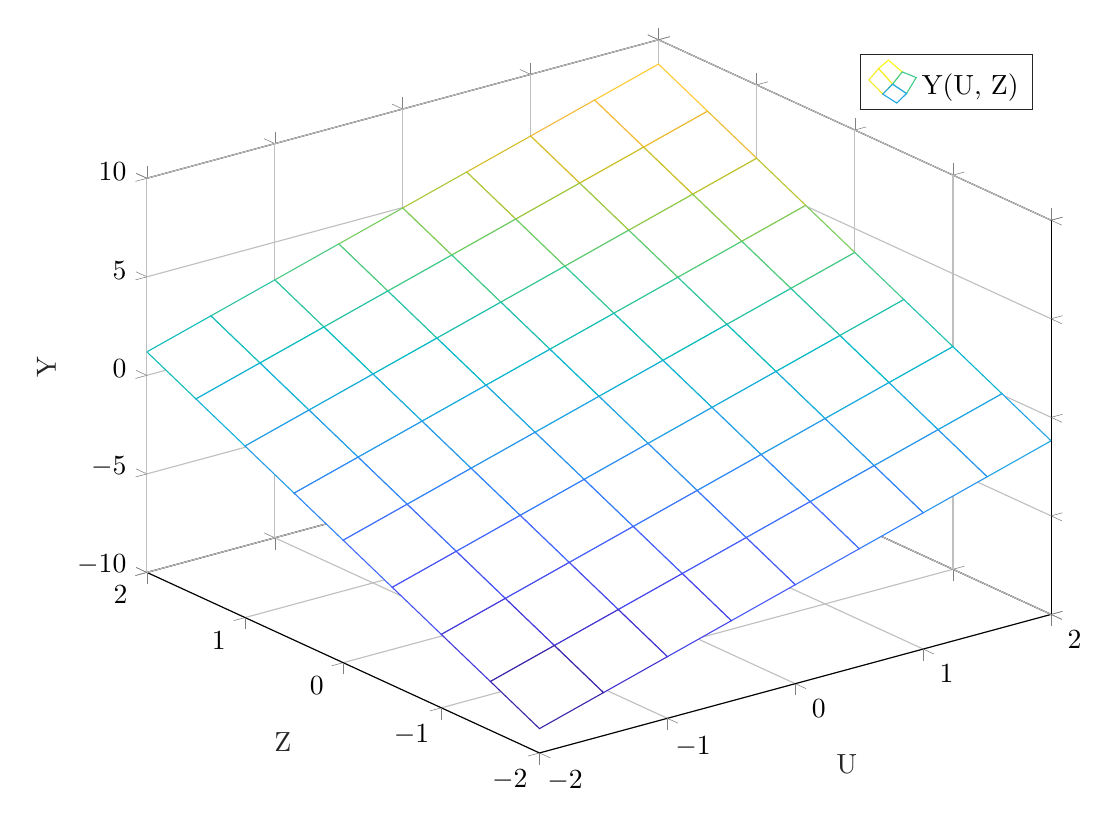
\begin{tikzpicture}

\begin{axis}[%
width=4.521in,
height=3.566in,
at={(0.758in,0.481in)},
scale only axis,
xmin=-2,
xmax=2,
tick align=outside,
xlabel style={font=\color{white!15!black}},
xlabel={U},
ymin=-2,
ymax=2,
ylabel style={font=\color{white!15!black}},
ylabel={Z},
zmin=-10,
zmax=10,
zlabel style={font=\color{white!15!black}},
zlabel={Y},
view={-37.5}{30},
axis background/.style={fill=white},
xmajorgrids,
ymajorgrids,
zmajorgrids,
legend style={legend cell align=left, align=left, draw=white!15!black}
]

\addplot3[%
surf,
shader=flat corner, fill=white, z buffer=sort, colormap={mymap}{[1pt] rgb(0pt)=(0.2422,0.1504,0.6603); rgb(1pt)=(0.25039,0.164995,0.707614); rgb(2pt)=(0.257771,0.181781,0.751138); rgb(3pt)=(0.264729,0.197757,0.795214); rgb(4pt)=(0.270648,0.214676,0.836371); rgb(5pt)=(0.275114,0.234238,0.870986); rgb(6pt)=(0.2783,0.255871,0.899071); rgb(7pt)=(0.280333,0.278233,0.9221); rgb(8pt)=(0.281338,0.300595,0.941376); rgb(9pt)=(0.281014,0.322757,0.957886); rgb(10pt)=(0.279467,0.344671,0.971676); rgb(11pt)=(0.275971,0.366681,0.982905); rgb(12pt)=(0.269914,0.3892,0.9906); rgb(13pt)=(0.260243,0.412329,0.995157); rgb(14pt)=(0.244033,0.435833,0.998833); rgb(15pt)=(0.220643,0.460257,0.997286); rgb(16pt)=(0.196333,0.484719,0.989152); rgb(17pt)=(0.183405,0.507371,0.979795); rgb(18pt)=(0.178643,0.528857,0.968157); rgb(19pt)=(0.176438,0.549905,0.952019); rgb(20pt)=(0.168743,0.570262,0.935871); rgb(21pt)=(0.154,0.5902,0.9218); rgb(22pt)=(0.146029,0.609119,0.907857); rgb(23pt)=(0.138024,0.627629,0.89729); rgb(24pt)=(0.124814,0.645929,0.888343); rgb(25pt)=(0.111252,0.6635,0.876314); rgb(26pt)=(0.0952095,0.679829,0.859781); rgb(27pt)=(0.0688714,0.694771,0.839357); rgb(28pt)=(0.0296667,0.708167,0.816333); rgb(29pt)=(0.00357143,0.720267,0.7917); rgb(30pt)=(0.00665714,0.731214,0.766014); rgb(31pt)=(0.0433286,0.741095,0.73941); rgb(32pt)=(0.0963952,0.75,0.712038); rgb(33pt)=(0.140771,0.7584,0.684157); rgb(34pt)=(0.1717,0.766962,0.655443); rgb(35pt)=(0.193767,0.775767,0.6251); rgb(36pt)=(0.216086,0.7843,0.5923); rgb(37pt)=(0.246957,0.791795,0.556743); rgb(38pt)=(0.290614,0.79729,0.518829); rgb(39pt)=(0.340643,0.8008,0.478857); rgb(40pt)=(0.3909,0.802871,0.435448); rgb(41pt)=(0.445629,0.802419,0.390919); rgb(42pt)=(0.5044,0.7993,0.348); rgb(43pt)=(0.561562,0.794233,0.304481); rgb(44pt)=(0.617395,0.787619,0.261238); rgb(45pt)=(0.671986,0.779271,0.2227); rgb(46pt)=(0.7242,0.769843,0.191029); rgb(47pt)=(0.773833,0.759805,0.16461); rgb(48pt)=(0.820314,0.749814,0.153529); rgb(49pt)=(0.863433,0.7406,0.159633); rgb(50pt)=(0.903543,0.733029,0.177414); rgb(51pt)=(0.939257,0.728786,0.209957); rgb(52pt)=(0.972757,0.729771,0.239443); rgb(53pt)=(0.995648,0.743371,0.237148); rgb(54pt)=(0.996986,0.765857,0.219943); rgb(55pt)=(0.995205,0.789252,0.202762); rgb(56pt)=(0.9892,0.813567,0.188533); rgb(57pt)=(0.978629,0.838629,0.176557); rgb(58pt)=(0.967648,0.8639,0.16429); rgb(59pt)=(0.96101,0.889019,0.153676); rgb(60pt)=(0.959671,0.913457,0.142257); rgb(61pt)=(0.962795,0.937338,0.12651); rgb(62pt)=(0.969114,0.960629,0.106362); rgb(63pt)=(0.9769,0.9839,0.0805)}, mesh/rows=9]
table[row sep=crcr, point meta=\thisrow{c}] {%
%
x	y	z	c\\
-2	-2	-8.7652	-8.7652\\
-2	-1.5	-7.5205	-7.5205\\
-2	-1	-6.2759	-6.2759\\
-2	-0.5	-5.0312	-5.0312\\
-2	0	-3.7865	-3.7865\\
-2	0.5	-2.5419	-2.5419\\
-2	1	-1.2972	-1.2972\\
-2	1.5	-0.052545	-0.052545\\
-2	2	1.1921	1.1921\\
-1.5	-2	-7.8186	-7.8186\\
-1.5	-1.5	-6.5739	-6.5739\\
-1.5	-1	-5.3292	-5.3292\\
-1.5	-0.5	-4.0846	-4.0846\\
-1.5	0	-2.8399	-2.8399\\
-1.5	0.5	-1.5952	-1.5952\\
-1.5	1	-0.35057	-0.35057\\
-1.5	1.5	0.89409	0.89409\\
-1.5	2	2.1388	2.1388\\
-1	-2	-6.8719	-6.8719\\
-1	-1.5	-5.6273	-5.6273\\
-1	-1	-4.3826	-4.3826\\
-1	-0.5	-3.1379	-3.1379\\
-1	0	-1.8933	-1.8933\\
-1	0.5	-0.6486	-0.6486\\
-1	1	0.59606	0.59606\\
-1	1.5	1.8407	1.8407\\
-1	2	3.0854	3.0854\\
-0.5	-2	-5.9253	-5.9253\\
-0.5	-1.5	-4.6806	-4.6806\\
-0.5	-1	-3.436	-3.436\\
-0.5	-0.5	-2.1913	-2.1913\\
-0.5	0	-0.94663	-0.94663\\
-0.5	0.5	0.29803	0.29803\\
-0.5	1	1.5427	1.5427\\
-0.5	1.5	2.7874	2.7874\\
-0.5	2	4.032	4.032\\
0	-2	-4.9787	-4.9787\\
0	-1.5	-3.734	-3.734\\
0	-1	-2.4893	-2.4893\\
0	-0.5	-1.2447	-1.2447\\
0	0	0	0\\
0	0.5	1.2447	1.2447\\
0	1	2.4893	2.4893\\
0	1.5	3.734	3.734\\
0	2	4.9787	4.9787\\
0.5	-2	-4.032	-4.032\\
0.5	-1.5	-2.7874	-2.7874\\
0.5	-1	-1.5427	-1.5427\\
0.5	-0.5	-0.29803	-0.29803\\
0.5	0	0.94663	0.94663\\
0.5	0.5	2.1913	2.1913\\
0.5	1	3.436	3.436\\
0.5	1.5	4.6806	4.6806\\
0.5	2	5.9253	5.9253\\
1	-2	-3.0854	-3.0854\\
1	-1.5	-1.8407	-1.8407\\
1	-1	-0.59606	-0.59606\\
1	-0.5	0.6486	0.6486\\
1	0	1.8933	1.8933\\
1	0.5	3.1379	3.1379\\
1	1	4.3826	4.3826\\
1	1.5	5.6273	5.6273\\
1	2	6.8719	6.8719\\
1.5	-2	-2.1388	-2.1388\\
1.5	-1.5	-0.89409	-0.89409\\
1.5	-1	0.35057	0.35057\\
1.5	-0.5	1.5952	1.5952\\
1.5	0	2.8399	2.8399\\
1.5	0.5	4.0846	4.0846\\
1.5	1	5.3292	5.3292\\
1.5	1.5	6.5739	6.5739\\
1.5	2	7.8186	7.8186\\
2	-2	-1.1921	-1.1921\\
2	-1.5	0.052545	0.052545\\
2	-1	1.2972	1.2972\\
2	-0.5	2.5419	2.5419\\
2	0	3.7865	3.7865\\
2	0.5	5.0312	5.0312\\
2	1	6.2759	6.2759\\
2	1.5	7.5205	7.5205\\
2	2	8.7652	8.7652\\
};
\addlegendentry{Y(U, Z)}

\end{axis}
\end{tikzpicture}%
    \caption{Charakterystyka statyczna obiektu y(u, z)}
    \label{projekt:zad2:charStat:figure}
\end{figure}

Wniosek: 

Na podstawie wykresu charakterystyki statycznej można ustalić, że właściwości
statyczne procesu są liniowe. Wzmocnienie statyczne procesu określone zostało dzieki …,
wynosi on K=1,0305.
